\documentclass[a4paper]{article}

\def\npart {IA}
\def\nterm {Michaelmas}
\def\nyear {2014}
\def\nlecturer {J.\ Goedecke}
\def\ncourse {Groups}

\input{header}

\begin{document}
\maketitle
{\small
  \noindent\textbf{Examples of groups}\\
  Axioms for groups. Examples from geometry: symmetry groups of regular polygons, cube, tetrahedron. Permutations on a set; the symmetric group. Subgroups and homomorphisms. Symmetry groups as subgroups of general permutation groups. The M\"obius group; cross-ratios, preservation of circles, the point at infinity. Conjugation. Fixed points of M\"obius maps and iteration.\hspace*{\fill} [4]

  \vspace{10pt}
  \noindent\textbf{Lagrange's theorem}\\
  Cosets. Lagrange's theorem. Groups of small order (up to order 8). Quaternions. Fermat-Euler theorem from the group-theoretic point of view.\hspace*{\fill} [5]

  \vspace{10pt}
  \noindent\textbf{Group actions}\\
  Group actions; orbits and stabilizers. Orbit-stabilizer theorem. Cayley's theorem (every group is isomorphic to a subgroup of a permutation group). Conjugacy classes. Cauchy's theorem.\hspace*{\fill} [4]

  \vspace{10pt}
  \noindent\textbf{Quotient groups}\\
  Normal subgroups, quotient groups and the isomorphism theorem.\hspace*{\fill} [4]

  \vspace{10pt}
  \noindent
  \textbf{Matrix groups}\\
  The general and special linear groups; relation with the M\"obius group. The orthogonal and special orthogonal groups. Proof (in $\R^3$) that every element of the orthogonal group is the product of reflections and every rotation in $\R^3$ has an axis. Basis change as an example of conjugation.\hspace*{\fill} [3]

  \vspace{10pt}
  \noindent\textbf{Permutations}\\
  Permutations, cycles and transpositions. The sign of a permutation. Conjugacy in $S_n$ and in $A_n$. Simple groups; simplicity of $A_5$.\hspace*{\fill} [4]}
\tableofcontents

\setcounter{section}{-1}
\section{Introduction}
Group theory is an example of \emph{algebra}. In pure mathematics, algebra (usually) does not refer to the boring mindless manipulation of symbols. Instead, in algebra, we have some set of objects with some operations on them. For example, we can take the integers with addition as the operation. However, in algebra, we allow \emph{any} set and \emph{any} operations, not just numbers.

Of course, such a definition is too broad to be helpful. We categorize algebraic structures into different types. In this course, we will study a particular kind of structures, \emph{groups}. In the IB Groups, Rings and Modules course, we will study rings and modules as well.

These different kinds of structures are defined by certain \emph{axioms}. The \emph{group axioms} will say that the operation must follow certain rules, and any set and operation that satisfies these rules will be considered to form a group. We will then have a different set of axioms for rings, modules etc.

As mentioned above, the most familiar kinds of algebraic structures are number systems such as integers and rational numbers. The focus of group theory, however, is not on things that resemble ``numbers''. Instead, it is the study of \emph{symmetries}.

First of all, what is a symmetry? We are all familiar with, say, the symmetries of an (equilateral) triangle (we will always assume the triangle is equilateral). We rotate a triangle by $120^\circ$, and we get the original triangle. We say that rotating by $120^\circ$ is a symmetry of a triangle. In general, a symmetry is something we do to an object that leaves the object intact.

Of course, we don't require that the symmetry leaves \emph{everything} intact. Otherwise, we would only be allowed to do nothing. Instead, we require certain important things to be intact. For example, when considering the symmetries of a triangle, we only care about how the resultant object looks, but don't care about where the individual vertices went.

In the case of the triangle, we have six symmetries: three rotations (rotation by $0^\circ, 120^\circ$ and $240^\circ$), and three reflections along the axes below:
\begin{center}
  \begin{tikzpicture}
    \foreach \x in {0,120,240} {
      \begin{scope}[rotate=\x]
        \draw (-1, -0.577) -- (1, -0.577);
        \draw [mred, dashed] (0, -1.2) -- (0, 1.778);
      \end{scope}
    }
  \end{tikzpicture}
\end{center}
These six together form the underlying set of the \emph{group of symmetries}. A more sophisticated example is the symmetries of $\R^3$. We define these as operations on $\R^3$ that leave distances between points unchanged. These include translations, rotations, reflections, and combinations of these.

So what is the operation? This operation combines two symmetries to give a new symmetry. The natural thing to do is to do the symmetry one after another. For example, if we combine the two $120^\circ$ rotations, we get a $240^\circ$ rotation.

Now we are studying algebra, not geometry. So to define the group, we \emph{abstract away} the triangle. Instead, we define the group to be six objects, say $\{e, r, r^2, s, rs, r^2s\}$, with rules defining how we combine two elements to get a third. Officially, we do not mention the triangle at all when defining the group.

We can now come up with the group axioms. What rules should the set of symmetries obey? First of all, we must have a ``do nothing'' symmetry. We call this the \emph{identity} element. When we compose the identity with another symmetry, the other symmetry is unchanged.

Secondly, given a symmetry, we can do the reverse symmetry. So for any element, there is an inverse element that, when combined with the original, gives the identity.

Finally, given three symmetries, we can combine them, one after another. If we denote the operation of the group as $*$, then if we have three symmetries, $x, y, z$, we should be able to form $x*y*z$. If we want to define it in terms of the binary operation $*$, we can define it as $(x*y)*z$, where we first combine the first two symmetries, then combine the result with the third. Alternatively, we can also define it as $x*(y*z)$. Intuitively, these two should give the same result, since both are applying $x$ after $y$ after $z$. Hence we have the third rule $x*(y*z) = (x*y)*z$.

Now a group is any set with an operation that satisfies the three rules above. In group theory, the objective is to study the properties of groups just assuming these three axioms. It turns out that there is a \emph{lot} we can talk about.

\section{Groups and homomorphisms}
\subsection{Groups}
\begin{defi}[Binary operation]
  A \emph{(binary) operation} on a set $A$ is a map $*\colon A \times A \rightarrow A$.
\end{defi}
\begin{defi}[Group]
  A \emph{group} is a set $G$ together with a binary operation $*$ on $G$ satisfying the following axioms:
  \begin{enumerate}[label=\arabic{*}.]
    \item There exists an element $e \in G$ such that for all $a \in G$,
      \[
        a*e = e*a = a.\tag{identity}
      \]
    \item For all $a \in G$, there exists an element $a^{-1} \in G$ such that
      \[
        a*a^{-1} = a^{-1}*a = e.\tag{inverse}
      \]
    \item For all $a, b, c\in G$,
      \[
        (a*b)*c = a*(b*c).\tag{associativity}
      \]
  \end{enumerate}
\end{defi}

\begin{defi}[Order of group]
  The \emph{order} of a group $G$, denoted by $|G|$, is the number of elements in $G$. A group is a \emph{finite group} if its order is finite.
\end{defi}

\begin{remark}
  Strictly speaking, the inverse axiom as stated is not yet well-defined, since we have not specified what $e$ is. The identity axiom only guarantees the existence of \emph{some} $e$ satisfying the identity property, but there could be many such elements. Thus, the inverse axiom should be interpreted as: for each $a \in G$, there exists $a^{-1} \in G$ such that $a*a^{-1}$ and $a^{-1} * a$ both satisfy the identity property. We will soon show that the identity is unique, after which this ambiguity is resolved.
\end{remark}

\begin{remark}
  Some authors include a zeroth axiom called \emph{closure}:
  \begin{enumerate}[label=\arabic{*}.]
      \setcounter{enumi}{-1}
    \item For all $a, b \in G$, we have $a * b \in G$.\hfill (closure)
  \end{enumerate}
  Since $*$ is defined to be a binary operation on $G$, this is automatically satisfied. However, in practice, one often needs to verify it explicitly. For example, if we let $G$ be the set of all matrices of the form
  \[
    \begin{pmatrix}
      1 & x & y\\
      0 & 1 & z\\
      0 & 0 & 1
    \end{pmatrix}
  \]
  under matrix multiplication, we must check that the product of two such matrices is again of this form. Formally, we are verifying that the binary operation is well-defined on $G$.
\end{remark}

\begin{remark}
  In general, it is \emph{not} the case that $a*b = b*a$ for all elements $a, b$ of a group $G$. For example, in the group of symmetries of a triangle, rotating and then reflecting is different from reflecting and then rotating.
\end{remark}

\begin{defi}[Abelian group]
  A group $(G, *)$ is \emph{abelian} if it additionally satisfies
  \begin{enumerate}[label=\arabic{*}.]
      \setcounter{enumi}{3}
    \item $(\forall a, b \in G)\, a*b = b*a$. \hfill (commutativity)
  \end{enumerate}
\end{defi}

\begin{notation}
  When the operation $*$ is clear from context, we write $ab$ in place of $a*b$. We also write $a^2 = aa$, $a^n = \underbrace{aaa\cdots a}_{n \text{ copies}}$, $a^0 = e$, and $a^{-n} = (a^{-1})^n$ for $n \geq 1$.
\end{notation}

\begin{eg}
  The following are abelian groups:
  \begin{enumerate}
    \item $(\Z, +)$
    \item $(\Q, +)$
    \item $(\Z_n, +_n)$, the integers modulo $n$ under addition modulo $n$
    \item $(\Q^*, \times)$, the nonzero rationals under multiplication
    \item $(\{-1, 1\}, \times)$
  \end{enumerate}
  The following are non-abelian groups:
  \begin{enumerate}[resume]
    \item The symmetry group of a regular $n$-gon under composition, denoted $D_{2n}$
    \item The group of $2\times 2$ invertible real matrices under matrix multiplication, denoted $\GL_2(\R)$
    \item Symmetry groups of 3D objects
  \end{enumerate}
\end{eg}

\begin{prop}[Uniqueness of identity and inverse]
  Let $(G, *)$ be a group. Then
  \begin{enumerate}
    \item The identity element is unique.
    \item For each $a \in G$, the inverse of $a$ is unique.
  \end{enumerate}
\end{prop}
\begin{proof}\leavevmode
  \begin{enumerate}[label=(\roman{*})]
    \item Suppose $e$ and $e'$ are both identity elements. Then $ee' = e'$, using the fact that $e$ is an identity, and $ee' = e$, using the fact that $e'$ is an identity. Thus $e = e'$.
    \item Suppose $a^{-1}$ and $b$ both satisfy the inverse axiom for some $a\in G$. Then $b = be = b(aa^{-1}) = (ba)a^{-1} = ea^{-1} = a^{-1}$. Thus $b = a^{-1}$.\qedhere
  \end{enumerate}
\end{proof}

\begin{remark}
  Since the identity is unique, it is now meaningful to speak of \emph{the} identity element $e$. Similarly, since inverses are unique, we may unambiguously write $a^{-1}$ for \emph{the} inverse of $a$.
\end{remark}

\begin{prop}[Inverse laws]
  Let $(G, *)$ be a group and let $a, b\in G$. Then
  \begin{enumerate}
    \item $(a^{-1})^{-1} = a$.
    \item $(ab)^{-1} = b^{-1}a^{-1}$.
  \end{enumerate}
\end{prop}
\begin{proof}\leavevmode
  \begin{enumerate}
    \item Given $a^{-1}$, both $a$ and $(a^{-1})^{-1}$ satisfy
      \[
        xa^{-1} = a^{-1}x = e.
      \]
      By uniqueness of inverses, $(a^{-1})^{-1} = a$.
    \item We have
      \begin{align*}
        (ab)(b^{-1}a^{-1}) &= a(bb^{-1})a^{-1} \\
        &= aea^{-1}\\
        &= aa^{-1}\\
        &= e
      \end{align*}
      Similarly, $(b^{-1}a^{-1})ab = e$. So $b^{-1}a^{-1}$ is an inverse of $ab$. By the uniqueness of inverses, $(ab)^{-1} = b^{-1}a^{-1}$.\qedhere
  \end{enumerate}
\end{proof}

\begin{defi}[Subgroup]
  Let $(G, *)$ be a group. A subset $H \subseteq G$ is a \emph{subgroup} of $G$, written $H\leq G$, if $H$ with the restricted operation $*$ from $G$ is itself a group.
\end{defi}

\begin{eg}\leavevmode
  \begin{itemize}
    \item $(\Z, +)\leq (\Q, +) \leq (\R, +)\leq (\C, +)$.
    \item $(\{e\}, *) \leq (G, *)$ for any group $G$ (the \emph{trivial subgroup}).
    \item $G \leq G$.
    \item $(\{\pm 1\}, \times) \leq (\Q^*, \times)$.
  \end{itemize}
\end{eg}

\begin{remark}
  To show that $H$ is a subgroup of $G$ directly from the definition, one must verify all the group axioms for $H$. The following two lemmas provide more convenient criteria.
\end{remark}

\begin{lemma}[Subgroup criteria I]
  Let $(G, *)$ be a group and let $H\subseteq G$. Then $H \leq G$ if and only if
  \begin{enumerate}
    \item $e \in H$;
    \item $(\forall a, b\in H)\,ab \in H$;
    \item $(\forall a \in H)\,a^{-1} \in H$.
  \end{enumerate}
\end{lemma}
\begin{proof}
  If $H \leq G$, then (i), (ii), and (iii) hold by the group axioms.

  Conversely, suppose (i), (ii), and (iii) hold. The group axioms for $H$ are then verified as follows:
  \begin{enumerate}[label=\arabic{*}.]
      \setcounter{enumi}{-1}
    \item Closure: by (ii).
    \item Identity: by (i). Note that $H$ and $G$ must have the same identity. Indeed, suppose $e_H$ and $e_G$ are the identities of $H$ and $G$ respectively. Then $e_He_H = e_H$. Since $e_H$ has an inverse $e_H^{-1}$ in $G$, multiplying on the right gives $e_H = e_G$.
    \item Inverse: by (iii).
    \item Associativity: inherited from $G$.\qedhere
  \end{enumerate}
\end{proof}

\begin{lemma}[Subgroup criteria II]
  Let $(G, *)$ be a group and let $H\subseteq G$. Then $H \leq G$ if and only if
  \begin{enumerate}[label=(\Roman{*})]
    \item $H$ is non-empty;
    \item $(\forall a, b\in H)\,ab^{-1}\in H$.
  \end{enumerate}
\end{lemma}
\begin{proof}
  If $H \leq G$, then (I) and (II) follow immediately from (i), (ii), and (iii) of Subgroup criteria~I.

  Conversely, suppose (I) and (II) hold. We verify conditions (i), (ii), and (iii):
  \begin{enumerate}
    \item Since $H$ is non-empty, it contains some element $a$. Then $aa^{-1} = e \in H$ by (II).
      \setcounter{enumi}{2}
    \item For any $a \in H$, we have $ea^{-1} = a^{-1} \in H$ by (II).
      \setcounter{enumi}{1}
    \item For any $a, b \in H$, since $b^{-1} \in H$ by (iii), we have $a(b^{-1})^{-1} = ab\in H$ by (II).
  \end{enumerate}
\end{proof}

\begin{prop}[Subgroups of $\Z$]
  The subgroups of $(\Z, +)$ are exactly the sets $n\Z = \{nk : k \in \Z\}$ for $n\in \N$.
\end{prop}
\begin{proof}
  For any $n \in \N$, it is straightforward to verify that $n\Z$ is a subgroup of $(\Z, +)$.

  Conversely, let $H\leq \Z$. We have $0\in H$. If $H = \{0\}$, then $H = 0\Z$ and we are done.

  Otherwise, $H$ contains a nonzero element $a$, and since $-a \in H$ as well, $H$ contains a positive integer. Let $n$ be the smallest positive integer in $H$. We claim that $H = n\Z$. Since $n \in H$ and $H$ is closed under addition and inverses, all multiples of $n$ belong to $H$, so $n\Z \subseteq H$. Now suppose for contradiction that there exists $a\in H$ with $n \nmid a$. By the division algorithm, write $a = pn + q$ where $0 < q < n$. Since $a - pn\in H$, we have $q\in H$. But $0 < q < n$, contradicting the minimality of $n$. Hence every element of $H$ is divisible by $n$, so $H \subseteq n\Z$. Therefore $H = n\Z$.
\end{proof}
\subsection{Homomorphisms}
\begin{remark}
  To study groups, it is essential to study structure-preserving functions between them. We first recall the basic definitions concerning functions.
\end{remark}

\begin{defi}[Function]
  Given two sets $X$ and $Y$, a \emph{function} $f\colon X \rightarrow Y$ sends each $x\in X$ to a particular element $f(x)\in Y$. The set $X$ is called the \emph{domain} and $Y$ is called the \emph{codomain}.
\end{defi}
\begin{eg}\leavevmode
  \begin{itemize}
    \item Identity function: for any set $X$, $1_X\colon X \rightarrow X$ with $1_X(x) = x$ is a function. This is also written as $\mathrm{id}_X$.
    \item Inclusion map: $\iota\colon \Z \rightarrow \Q$ defined by $\iota(n) = n$. Note that this differs from the identity function, as the domain and codomain are different.
    \item $f_1\colon \Z \rightarrow \Z$ defined by $f_1(x) = x + 1$.
    \item $f_2\colon \Z \rightarrow \Z$ defined by $f_2(x) = 2x$.
    \item $f_3\colon \Z \rightarrow \Z$ defined by $f_3(x) = x^2$.
    \item Consider functions $\{0, 1, 2, 3, 4\} \rightarrow \{0, 1, 2, 3, 4\}$:
      \begin{itemize}
        \item $g_1(x) = x + 1$ if $x < 4$; $g_1(4) = 4$.
        \item $g_2(x) = x + 1$ if $x < 4$; $g_2(4) = 0$.
      \end{itemize}
  \end{itemize}
\end{eg}
\begin{defi}[Composition of functions]
  Let $f\colon X \rightarrow Y$ and $g\colon Y\rightarrow Z$ be functions. The \emph{composition} of $g$ with $f$ is the function $g\circ f\colon X \rightarrow Z$ defined by $(g\circ f)(x) = g(f(x))$.
\end{defi}
\begin{eg}
  Using $f_1$ and $f_2$ defined above, $(f_2\circ f_1)(x) = 2x + 2$ and $(f_1\circ f_2)(x) = 2x + 1$. Note that function composition is not commutative in general.
\end{eg}
\begin{defi}[Injective function]
  A function $f\colon X \to Y$ is \emph{injective} if distinct elements have distinct images, i.e.
  \[
    (\forall x, y\in X)\,f(x) = f(y)\Rightarrow x = y.
  \]
\end{defi}

\begin{defi}[Surjective function]
  A function $f\colon X \to Y$ is \emph{surjective} if every element of $Y$ is in the image of $f$, i.e.
  \[
    (\forall y\in Y)(\exists x\in X)\,f(x) = y.
  \]
\end{defi}

\begin{defi}[Bijective function]
  A function $f\colon X \to Y$ is \emph{bijective} if it is both injective and surjective. A function has an inverse if and only if it is bijective.
\end{defi}

\begin{eg}
  $\iota$ and $f_2$ are injective but not surjective. $f_3$ and $g_1$ are neither. $1_X$, $f_1$ and $g_2$ are bijective.
\end{eg}

\begin{lemma}[Composition of bijections]
  The composition of two bijective functions is bijective.
\end{lemma}

\begin{remark}
  When studying groups, we are not interested in arbitrary functions between the underlying sets. Instead, we consider functions that preserve the group structure, called \emph{homomorphisms}.
\end{remark}

\begin{defi}[Group homomorphism]
  Let $(G, *)$ and $(H, \times)$ be groups. A function $f\colon G\rightarrow H$ is a \emph{group homomorphism} if
  \[
   ( \forall g_1, g_2 \in G)\, f(g_1)\times f(g_2) = f(g_1 * g_2).
  \]
\end{defi}

\begin{defi}[Group isomorphism]
  A \emph{group isomorphism} is a bijective group homomorphism. Two groups $G$ and $H$ are \emph{isomorphic}, written $G\cong H$, if there exists an isomorphism between them.
\end{defi}

\begin{remark}
  Isomorphic groups are considered to be ``the same'' from a group-theoretic perspective. For example, when we say that there is only one group of order $2$, we mean that any two groups of order $2$ are isomorphic.
\end{remark}

\begin{eg}\leavevmode
  \begin{itemize}
    \item For any groups $G$ and $H$, the function $f\colon G \to H$ defined by $f(g) = e_H$ for all $g \in G$ is a homomorphism (the \emph{trivial homomorphism}).
    \item $1_G\colon G \rightarrow G$ and $f_2\colon \Z \rightarrow 2\Z$ are isomorphisms. $\iota\colon \Z\rightarrow\Q$ and $f_2\colon\Z\rightarrow\Z$ are homomorphisms.
    \item $\exp\colon (\R, +) \rightarrow (\R^+, \times)$ defined by $\exp(x) = e^x$ is an isomorphism.
    \item Let $H = (\{e^{ik\pi/2}:k=0, 1 ,2, 3\}, \times)$. Then $f\colon \Z_4 \rightarrow H$ defined by $f(a) = e^{i\pi a/2}$ is an isomorphism.
    \item $\det\colon \GL_2(\R) \rightarrow \R^*$ is a homomorphism.
  \end{itemize}
\end{eg}

\begin{prop}[Elementary homomorphism properties]
  Let $f\colon G\rightarrow H$ be a group homomorphism. Then
  \begin{enumerate}
    \item $f(e_G) = e_H$.
    \item For all $a \in G$, $f(a^{-1}) = f(a)^{-1}$.
    \item The composite of two group homomorphisms is a group homomorphism.
    \item The inverse of an isomorphism is an isomorphism.
  \end{enumerate}
\end{prop}
\begin{proof}\leavevmode
  \begin{enumerate}
    \item \begin{align*}
        f(e_G) &= f(e_G^2) = f(e_G)^2\\
        f(e_G)^{-1}f(e_G) &= f(e_G)^{-1}f(e_G)^2\\
        f(e_G) &= e_H
      \end{align*}
    \item \begin{align*}
        e_H &= f(e_G)\\
        &= f(aa^{-1})\\
        &= f(a)f(a^{-1})
      \end{align*}
      Since inverses are unique, $f(a^{-1}) = f(a)^{-1}$.
    \item Let $f\colon G_1 \rightarrow G_2$ and $g\colon G_2 \rightarrow G_3$ be homomorphisms. Then $g(f(ab)) = g(f(a)f(b)) = g(f(a))g(f(b))$.
    \item Let $f\colon G \rightarrow H$ be an isomorphism and let $a, b \in H$. Then
      \begin{align*}
        f^{-1}(ab) &= f^{-1}\Big\{f\big[f^{-1}(a)\big]f\big[f^{-1}(b)\big]\Big\}\\
        &= f^{-1}\Big\{f\big[f^{-1}(a)f^{-1}(b)\big]\Big\}\\
        &= f^{-1}(a)f^{-1}(b)
      \end{align*}
      So $f^{-1}$ is a homomorphism. Since it is bijective, $f^{-1}$ is an isomorphism.\qedhere
  \end{enumerate}
\end{proof}

\begin{defi}[Image of homomorphism]
  Let $f\colon G\rightarrow H$ be a group homomorphism. The \emph{image} of $f$ is
  \[
    \im f = f(G) = \{f(g):g\in G\}.
  \]
\end{defi}

\begin{defi}[Kernel of homomorphism]
  Let $f\colon G\rightarrow H$ be a group homomorphism. The \emph{kernel} of $f$ is
  \[
    \ker f = f^{-1}(\{e_H\}) = \{g\in G:f(g)=e_H\}.
  \]
\end{defi}

\begin{prop}[Image and kernel subgroup property]
  Let $f\colon G \to H$ be a group homomorphism. Then $\im f\leq H$ and $\ker f \leq G$.
\end{prop}

\begin{proof}
  Since $f(e_G) = e_H$, we have $e_H\in \im f$ and $e_G\in \ker f$, so both sets are non-empty. For the image, suppose $b_1, b_2\in \im f$, so there exist $a_1, a_2 \in G$ with $f(a_1) = b_1$ and $f(a_2) = b_2$. Then $b_1b_2^{-1} = f(a_1)f(a_2)^{-1} = f(a_1 a_2^{-1})\in \im f$.

  For the kernel, suppose $b_1,b_2\in \ker f$. Then $f(b_1b_2^{-1}) = f(b_1)f(b_2)^{-1} = e_H e_H^{-1} = e_H$, so $b_1b_2^{-1}\in \ker f$.
\end{proof}

\begin{prop}[Kernel conjugation closure]
  Let $f\colon G\rightarrow H$ be a group homomorphism. Then for all $a\in G$ and all $k\in \ker f$, we have $aka^{-1}\in\ker f$.
\end{prop}

\begin{proof}
  $f(aka^{-1}) = f(a)f(k)f(a)^{-1} = f(a)e_Hf(a)^{-1} = e_H$. So $aka^{-1}\in \ker f$.
\end{proof}

\begin{remark}
  The above property---that $aka^{-1} \in \ker f$ for all $a \in G$ and $k \in \ker f$---is not special to kernels. Subgroups satisfying this property are called \emph{normal subgroups} and play a central role in the theory, as we will see later.
\end{remark}

\begin{eg}
  Images and kernels for previously defined homomorphisms:
  \begin{enumerate}
    \item For the trivial homomorphism $f\colon G \to H$ with $f(g) = e_H$, we have $\im f = \{e_H\}$ and $\ker f = G$.
    \item For the identity function, $\im 1_G = G$ and $\ker 1_G = \{e\}$.
    \item For the inclusion map $\iota\colon \Z\rightarrow\Q$, we have $\im \iota = \Z$ and $\ker \iota = \{0\}$.
    \item For $f_2\colon\Z\rightarrow\Z$ defined by $f_2(x) = 2x$, we have $\im f_2 = 2\Z$ and $\ker f_2 = \{0\}$.
    \item For $\det\colon \GL_2(\R) \rightarrow \R^*$, we have $\im \det = \R^*$ and $\ker \det = \{A \in \GL_2(\R):\det A = 1\} = \SL_2(\R)$.
  \end{enumerate}
\end{eg}

\begin{prop}[Injectivity and surjectivity criterion]
  Let $f\colon G\rightarrow H$ be a group homomorphism. Then $f$ is
  \begin{enumerate}
    \item surjective if and only if $\im f = H$;
    \item injective if and only if $\ker f = \{e_G\}$.
  \end{enumerate}
\end{prop}

\begin{proof}\leavevmode
  \begin{enumerate}
    \item This follows directly from the definitions.
    \item Since $f(e_G) = e_H$, we have $e_G \in \ker f$. If $f$ is injective, then $e_G$ is the only element mapping to $e_H$, so $\ker f = \{e_G\}$. Conversely, if $\ker f = \{e_G\}$, then given $a, b \in G$ with $f(a) = f(b)$, we have $f(ab^{-1}) = f(a)f(b)^{-1} = e_H$. Thus $ab^{-1}\in \ker f = \{e_G\}$, so $ab^{-1} = e_G$ and hence $a = b$.\qedhere
  \end{enumerate}
\end{proof}

\begin{remark}
  The image and kernel of a homomorphism are not merely convenient terminology. They are related by the \emph{first isomorphism theorem}, which we will prove after developing some further theory.
\end{remark}

\subsection{Cyclic groups}
\begin{remark}
  The simplest class of groups is that of \emph{cyclic groups}. Informally, a cyclic group is a group of the form $\{e, a, a^2, a^3, \ldots, a^{n - 1}\}$, where $a^n = e$. For example, the group of rotations of an equilateral triangle is $\{e, r, r^2\}$ where $r$ denotes rotation by $120^\circ$ and $r^3 = e$.
\end{remark}

\begin{defi}[Cyclic group]
  A group $G$ is \emph{cyclic} if
  \[
    (\exists a \in G)(\forall b \in G)(\exists n\in\Z)\, b = a^n,
  \]
  i.e.\ every element of $G$ is a power of $a$. Such an element $a$ is called a \emph{generator} of $G$.

  We write $C_n$ for the cyclic group of order $n$.
\end{defi}

\begin{eg}\leavevmode
  \begin{enumerate}
    \item $(\Z, +)$ is cyclic with generator $1$ (or $-1$). It is \emph{the} infinite cyclic group.
    \item $(\{+1, -1\}, \times)$ is cyclic with generator $-1$.
    \item $(\Z_n, +)$ is cyclic; its generators are precisely the elements coprime to $n$.
  \end{enumerate}
\end{eg}

\begin{notation}
  Given a group $G$ and an element $a\in G$, we write $\langle a\rangle$ for the \emph{cyclic subgroup generated by $a$}, i.e.\ the subgroup of all powers of $a$. It is the smallest subgroup of $G$ containing $a$.
\end{notation}

\begin{defi}[Order of element]
  Let $G$ be a group and let $a \in G$. The \emph{order} of $a$, denoted $\ord(a)$, is the smallest positive integer $n$ such that $a^n = e$. If no such $n$ exists, we say $a$ has \emph{infinite order}.
\end{defi}

\begin{remark}
  The word ``order'' now has two meanings: the order of a group ($|G|$) and the order of an element ($\ord(a)$). The following lemma shows that these are closely related.
\end{remark}

\begin{lemma}[Order equals cyclic subgroup size]
  Let $G$ be a group and let $a \in G$. Then $\ord (a) = |\langle a\rangle|$.
\end{lemma}
\begin{proof}
  If $\ord (a) = \infty$, then $a^n \neq a^m$ for all $n\neq m$ (otherwise $a^{m-n} = e$, contradicting infinite order). Thus $|\langle a\rangle| = \infty = \ord (a)$.

  Otherwise, suppose $\ord (a) = k$, so that $a^k = e$. We claim that $\langle a\rangle = \{e, a, a^2, \ldots, a^{k-1}\}$. Since $a^k = e$, every power of $a$ reduces to one of $e, a, \ldots, a^{k-1}$, so $\langle a \rangle$ contains no additional elements. Moreover, these $k$ elements are distinct: if $a^m = a^n$ for $0 \leq n < m \leq k - 1$, then $a^{m-n} = e$ with $0 < m - n < k$, contradicting the minimality of $k$. Hence $|\langle a\rangle| = k = \ord(a)$.
\end{proof}

\begin{prop}[Cyclic group commutativity]
  Every cyclic group is abelian.
\end{prop}
\begin{proof}
  Let $G = \langle a \rangle$ be cyclic. For any $b, c \in G$, we have $b = a^m$ and $c = a^n$ for some $m, n \in \Z$. Then $bc = a^m a^n = a^{m+n} = a^n a^m = cb$.
\end{proof}

\begin{defi}[Exponent of group]
  The \emph{exponent} of a group $G$ is the smallest positive integer $n$ such that $a^n = e$ for all $a \in G$.
\end{defi}

\subsection{Dihedral groups}
\begin{defi}[Dihedral group $D_{2n}$]
  For $n \geq 3$, the \emph{dihedral group} $D_{2n}$ is the group of symmetries of a regular $n$-gon. It has order $2n$, consisting of $n$ rotations (including the identity) and $n$ reflections, and admits the presentation
  \begin{align*}
    D_{2n} &= \langle r, s\mid r^n=s^2=e,\, srs^{-1} = r^{-1}\rangle\\
    &= \{e, r, r^2, \ldots, r^{n-1}, s, rs, r^2s, \ldots, r^{n-1}s\}.
  \end{align*}
  The subscript in $D_{2n}$ refers to the order of the group, not the number of sides of the polygon.
\end{defi}

\begin{remark}
  Geometrically, $r$ represents rotation by $360^\circ/n$ (which has order $n$) and $s$ represents a fixed reflection (which has order $2$). The relation $srs^{-1} = r^{-1}$ expresses the fact that conjugating a rotation by a reflection reverses the direction of rotation. Every element of $D_{2n}$ can be written uniquely in the form $r^m$ (a rotation) or $r^m s$ (a reflection) for $0 \leq m \leq n - 1$.
\end{remark}

\begin{notation}
  The notation $\langle \text{generators} \mid \text{relations} \rangle$ is called a \emph{group presentation}. For example, the cyclic group of order $n$ can be written as
  \[
    C_n = \langle a\mid a^n = e \rangle.
  \]
\end{notation}

\subsection{Direct products of groups}
\begin{defi}[Direct product of groups]
  Given two groups $(G, \circ)$ and $(H, \bullet)$, the \emph{direct product} $G\times H$ is the set of ordered pairs $\{(g, h) : g\in G,\, h\in H\}$ equipped with the componentwise operation
  \[
    (a_1, a_2)*(b_1, b_2) = (a_1\circ b_1,\, a_2\bullet b_2).
  \]
  This is a group with identity $(e_G, e_H)$ and inverses $(g, h)^{-1} = (g^{-1}, h^{-1})$.
\end{defi}

\begin{remark}
  The direct product arises naturally when considering symmetries of independent objects. For example, the symmetry group of a system of two independent equilateral triangles is $D_6 \times D_6$.
\end{remark}

\begin{eg}
  \begin{align*}
    C_2\times C_2 &= \{(0, 0), (0, 1), (1, 0), (1, 1)\}\\
    &= \{e, x, y, xy\} \text{ with every non-identity element of order 2}\\
    &= \langle x, y\mid x^2=y^2=e,\, xy = yx\rangle.
  \end{align*}
\end{eg}

\begin{prop}[Cyclic direct product criterion]
  $C_n\times C_m\cong C_{nm}$ if and only if $\hcf(m, n) = 1$.
\end{prop}

\begin{proof}
  Suppose that $\hcf(m, n) = 1$. Let $C_n = \langle a\rangle$ and $C_m = \langle b \rangle$, and let $k = \ord((a, b))$ in $C_n \times C_m$. Then $(a, b)^k = (a^k, b^k) = (e, e)$, which requires $n \mid k$ and $m \mid k$, i.e.\ $k$ is a common multiple of $n$ and $m$. Since $k$ is the smallest such positive integer, $k = \lcm(n, m) = \frac{nm}{\hcf(n, m)} = nm$.

  Now $\langle (a, b)\rangle \leq C_n\times C_m$, and since $(a, b)$ has order $nm = |C_n\times C_m|$, we have $\langle (a, b)\rangle = C_n\times C_m$. Thus $C_n\times C_m$ is cyclic of order $nm$, so $C_n\times C_m \cong C_{nm}$.

  Conversely, suppose $\hcf(m, n) \neq 1$. Let $k = \lcm(m, n) < mn$. Then for any $(a, b)\in C_n \times C_m$, we have $(a, b)^k = (a^k, b^k) = (e, e)$, so the order of every element divides $k < mn$. In particular, no element has order $mn$, so $C_n\times C_m$ is not cyclic of order $mn$.
\end{proof}

\begin{remark}
  Given a group $G$, it is sometimes useful to recognise it as a direct product of two of its subgroups. The following proposition gives a criterion for doing so.
\end{remark}

\begin{prop}[Direct product theorem]
  Let $G$ be a group and let $H_1, H_2\leq G$. Suppose:
  \begin{enumerate}
    \item $H_1\cap H_2 = \{e\}$;
    \item $(\forall a_1\in H_1)(\forall a_2 \in H_2)\, a_1a_2=a_2a_1$;
    \item $(\forall a\in G)(\exists a_1\in H_1)(\exists a_2 \in H_2)\,a = a_1a_2$ (i.e.\ $G=H_1H_2$).
  \end{enumerate}
  Then $G\cong H_1\times H_2$.
\end{prop}

\begin{proof}
  Define $f\colon H_1\times H_2\rightarrow G$ by $f(a_1, a_2) = a_1a_2$. This is a homomorphism, since by (ii),
  \begin{align*}
    f((a_1, a_2)*(b_1,b_2)) &= f(a_1b_1, a_2b_2)\\
    &= a_1b_1a_2b_2\\
    &= a_1a_2b_1b_2\\
    &= f(a_1, a_2)\,f(b_1,b_2).
  \end{align*}
  Surjectivity follows from (iii). For injectivity, suppose $f(a_1, a_2)=e$, i.e.\ $a_1a_2 = e$. Then $a_1=a_2^{-1}$. Since $a_1 \in H_1$ and $a_2^{-1} \in H_2$, we have $a_1 = a_2^{-1} \in H_1\cap H_2 = \{e\}$ by (i). Thus $a_1 = a_2 = e$, so $\ker f = \{e\}$ and $f$ is injective.
\end{proof}

\section{Symmetric group I}
\begin{remark}
  Recall that a symmetry of an object is a bijection that preserves some structure. For example, a symmetry of $\R^2$ is a bijection $f\colon \R^2 \to \R^2$ that preserves distances. We now consider the case where no structure needs to be preserved: the group of \emph{all} bijections from a set to itself. This is the \emph{symmetric group}, and it is in some sense the most general symmetry group. We will later show (in Chapter~\ref{sec:action}) that every group is isomorphic to a subgroup of some symmetric group.
\end{remark}

\subsection{Symmetric groups}
\begin{defi}[Permutation]
  Let $X$ be a set. A \emph{permutation} of $X$ is a bijection $\sigma\colon X \to X$. The set of all permutations of $X$ is denoted $\Sym X$.
\end{defi}

\begin{remark}
  We compose permutations as functions: if $\sigma$ and $\tau$ are permutations, then $\sigma\circ \tau$ denotes first applying $\tau$, then applying $\sigma$.
\end{remark}

\begin{thm}[Symmetric group]
  $(\Sym X, \circ)$ is a group.
\end{thm}

\begin{proof}
  The group axioms are verified as follows:
  \begin{enumerate}[label=\arabic{*}.]
      \setcounter{enumi}{-1}
    \item If $\sigma, \tau\in \Sym X$, then $\sigma\circ\tau\colon X\to X$ is a bijection, so $\sigma\circ\tau\in\Sym X$.
    \item The identity function $1_X\colon X\to X$ is a permutation and satisfies $\sigma \circ 1_X = 1_X \circ \sigma = \sigma$ for all $\sigma \in \Sym X$.
    \item Every bijection has a bijective inverse, so if $\sigma\in \Sym X$, then $\sigma^{-1} \in \Sym X$.
    \item Composition of functions is associative.\qedhere
  \end{enumerate}
\end{proof}

\begin{defi}[Symmetric group $S_n$]
  If $X$ is a finite set with $|X| = n$ (we usually take $X = \{1, 2, \ldots, n\}$), we write $S_n = \Sym X$. This is the \emph{symmetric group} of degree $n$.
\end{defi}

\begin{remark}
  The \emph{degree} of $S_n$ is $n$, while the \emph{order} of $S_n$ is $|S_n| = n!$. For example, $S_3$ has degree $3$ but order $6$.
\end{remark}

\begin{notation}[Two row notation]
  A permutation $\sigma \in S_n$ can be written by listing $1, 2, \ldots, n$ on the top row and their images below:
  \[
    \begin{pmatrix}
      1 & 2 & 3 &\cdots& n\\
      \sigma(1) & \sigma(2)&\sigma(3) &\cdots& \sigma(n)
    \end{pmatrix}.
  \]
  For example,
  \[
    \begin{pmatrix}
      1 & 2 & 3\\
      2 & 3 & 1
    \end{pmatrix}\in S_3 \quad\text{and}\quad
    \begin{pmatrix}
      1 & 2 & 3 & 4 & 5\\
      2 & 1 & 3 & 4 & 5
    \end{pmatrix}\in S_5.
  \]
\end{notation}

\begin{eg}
  For small values of $n$:
  \begin{enumerate}
    \item $S_1 = \left\{\begin{pmatrix}1\\1\end{pmatrix}\right\} = \{e\}\cong C_1$.
    \item $S_2 = \left\{\begin{pmatrix}1 & 2\\ 1 & 2\end{pmatrix}, \begin{pmatrix}1 & 2\\2 & 1\end{pmatrix}\right\}\cong C_2$.
    \item $S_3 = \left\{\begin{matrix}\begin{pmatrix}1 & 2 & 3\\1 & 2 & 3\end{pmatrix}, &\begin{pmatrix}1 & 2 & 3\\ 2 & 3 & 1\end{pmatrix}, &\begin{pmatrix}1 & 2 & 3\\3 & 1 & 2\end{pmatrix}\\\\\begin{pmatrix}1 & 2 & 3\\2 & 1 & 3\end{pmatrix}, &\begin{pmatrix}1 & 2 & 3\\ 3 & 2 & 1\end{pmatrix}, &\begin{pmatrix}1 & 2 & 3\\1 & 3 & 2\end{pmatrix}\end{matrix}\right\}\cong D_6$.
  \end{enumerate}
\end{eg}

\begin{remark}
  $S_3$ is not abelian, and hence $S_n$ is not abelian for any $n \geq 3$, since $S_3$ can be viewed as a subgroup of $S_n$ (by fixing $4, 5, \ldots, n$). More generally, $D_{2n}$ can be viewed as a subgroup of $S_n$, since each symmetry of a regular $n$-gon permutes its vertices.
\end{remark}

\begin{notation}[Cycle notation]
  A permutation that sends $a_1 \mapsto a_2 \mapsto \cdots \mapsto a_k \mapsto a_1$ and fixes all other elements is written as the cycle $(a_1\; a_2\; \cdots\; a_k)$. By convention, we write the smallest element first and omit fixed points. More general permutations can be written as products of cycles; for example, $(1\; 2)(3\; 4) \in S_4$ denotes the permutation that swaps $1$ with $2$ and $3$ with $4$.
\end{notation}

\begin{prop}[Cycle inverse]
  The inverse of a cycle is obtained by writing it in reverse order, e.g.\ $(1\; 2\; 3)^{-1} = (3\; 2\; 1) = (1\; 3\; 2)$.
\end{prop}

\begin{eg}\leavevmode
  \begin{enumerate}
    \item $(1\; 2\; 3)(1\; 2) = (1\;3)$, since (composing right to left) $1 \mapsto 2 \mapsto 3$, $3 \mapsto 3 \mapsto 1$, and $2 \mapsto 1 \mapsto 2$.
    \item $(1\; 2\; 3\; 4)(1\; 4) = (2\; 3\; 4)$.
  \end{enumerate}
\end{eg}

\begin{defi}[$k$-cycles and transpositions]
  A cycle $(a_1\; a_2\; \cdots\; a_k)$ is called a \emph{$k$-cycle}. A $2$-cycle is called a \emph{transposition}. Two cycles are \emph{disjoint} if no element appears in both.
\end{defi}

\begin{eg}
  $(1\; 2)$ and $(3\; 4)$ are disjoint, but $(1\; 2\; 3)$ and $(1\; 2)$ are not.
\end{eg}

\begin{lemma}[Disjoint cycle commutativity]
  Disjoint cycles commute.
\end{lemma}
\begin{proof}
  Let $\sigma, \tau\in S_n$ be disjoint cycles. We show that $\sigma(\tau(a)) = \tau(\sigma(a))$ for all $a \in \{1, \ldots, n\}$. If $a$ appears in neither $\sigma$ nor $\tau$, then both sides equal $a$. Otherwise, assume without loss of generality that $a$ appears in $\tau$ but not in $\sigma$. Then $\tau(a)$ also appears in $\tau$ and hence not in $\sigma$, so $\sigma(\tau(a)) = \tau(a)$. On the other hand, $\sigma(a) = a$, so $\tau(\sigma(a)) = \tau(a)$. Thus $\sigma \circ \tau = \tau \circ \sigma$.
\end{proof}

\begin{remark}
  Non-disjoint cycles need not commute. For example, $(1\; 3)(2\; 3) = (1\; 3\; 2)$ while $(2\; 3)(1\; 3) = (1\; 2\; 3)$.
\end{remark}

\begin{thm}[Disjoint cycle decomposition]
  Every permutation in $S_n$ can be written as a product of disjoint cycles. This decomposition is unique up to the ordering of cycles and cyclic rotation within each cycle.
\end{thm}

\begin{proof}
  Let $\sigma\in S_n$. Form the sequence $1, \sigma(1), \sigma^2(1), \sigma^3(1), \ldots$ Since the set $\{1, 2, \ldots, n\}$ is finite, for some $k$ we must have $\sigma^k(1)$ equal to a previous term. If $\sigma^k(1) = \sigma^l(1)$ with $l < k$, then $\sigma^{k-l}(1) = 1$. So all terms $\sigma^i(1)$ are distinct until we return to $1$, giving the first cycle $(1\; \sigma(1)\; \sigma^2(1)\;\cdots\;\sigma^{k-1}(1))$.

  Now choose the smallest element not yet in any cycle, say $j$, and repeat to obtain a cycle $(j\; \sigma(j)\; \sigma^2(j)\;\cdots\; \sigma^{l - 1}(j))$. Since $\sigma$ is a bijection, no element of this cycle can appear in a previous cycle.

  Repeat until all elements of $\{1, 2, \ldots, n\}$ are exhausted. Uniqueness holds because each element $j$ determines the cycle it belongs to: it must be $(j\; \sigma(j)\; \sigma^2(j)\; \cdots)$, regardless of which element we start with.
\end{proof}

\begin{defi}[Cycle type]
  Let $\sigma\in S_n$ and write $\sigma$ in disjoint cycle notation. The \emph{cycle type} of $\sigma$ is the list of cycle lengths, which is unique up to reordering. By convention, we often omit $1$-cycles (fixed points).
\end{defi}

\begin{eg}
  $(1\; 2)$ has cycle type $2$ (a transposition). $(1\; 2)(3\; 4)$ has cycle type $2, 2$ (a double transposition). $(1\; 2\; 3)(4\; 5)$ has cycle type $3, 2$.
\end{eg}

\begin{lemma}[Order of a permutation]
  Let $\sigma\in S_n$, and write $\sigma$ as a product of disjoint cycles. Then the order of $\sigma$ is the least common multiple of the cycle lengths. In particular, a $k$-cycle has order $k$.
\end{lemma}

\begin{proof}
  Write $\sigma = \tau_1\tau_2\cdots\tau_l$ where the $\tau_i$ are disjoint cycles. Since disjoint cycles commute, $\sigma^m = \tau_1^m\tau_2^m\cdots\tau_l^m$ for all $m \geq 1$.

  If $\tau_i$ has length $k_i$, then $\tau_i^m = e$ if and only if $k_i \mid m$. Thus $\sigma^m = e$ if and only if $k_i \mid m$ for all $i$, i.e.\ $m$ is a common multiple of $k_1, \ldots, k_l$. The order of $\sigma$ is therefore $\lcm(k_1, \ldots, k_l)$.
\end{proof}

\begin{eg}
  Any transposition or double transposition has order $2$. The permutation $(1\; 2\; 3)(4\; 5)$ has order $\lcm(3, 2) = 6$.
\end{eg}

\subsection{Sign of permutations}
\begin{remark}
  While classifying permutations by cycle type is very useful, it is a rather fine division. In this section, we assign a coarser invariant---the \emph{sign}---to each permutation, classifying it as either even or odd.
\end{remark}

\begin{prop}[Transposition generation]
  Every permutation in $S_n$ is a product of transpositions.
\end{prop}

\begin{proof}
  Since every permutation is a product of disjoint cycles, it suffices to show that each cycle is a product of transpositions. Indeed, $(a_1\; a_2\; a_3\; \cdots\; a_k) = (a_1\; a_2)(a_2\; a_3)\cdots (a_{k-1}\; a_k)$, so a $k$-cycle is a product of $k - 1$ transpositions.
\end{proof}

\begin{remark}
  The decomposition into transpositions is not unique. For example,
  \[
    (1\; 2\; 3\; 4\; 5) =(1\; 2)(2\; 3)(3\; 4)(4\; 5) = (1\; 2)(2\; 3)(1\; 2)(3\; 4)(1\; 2)(4\; 5).
  \]
  However, the parity (even or odd) of the number of transpositions is always the same, as the following theorem shows.
\end{remark}

\begin{thm}[Parity of transposition decomposition]
  Let $\sigma\in S_n$. If $\sigma$ is written as a product of transpositions in two different ways, then the number of transpositions in each decomposition has the same parity (both even or both odd).
\end{thm}

\begin{proof}
  For $\sigma \in S_n$, write $\#(\sigma)$ for the number of cycles in the disjoint cycle notation of $\sigma$, including $1$-cycles. So $\#(e) = n$ and $\#((1\; 2)) = n - 1$. We claim that for any transposition $\tau$, $\#(\sigma\tau) \equiv \#(\sigma) + 1 \pmod 2$.

  Let $\tau = (c\; d)$ with $c < d$.
  \begin{itemize}
    \item If $c$ and $d$ are in the same cycle of $\sigma$, say $(c\; a_2\; \cdots \; a_{k - 1}\; d\; a_{k + 1}\; \cdots\; a_{k + l})$, then
    \[
      (c\; a_2\; \cdots \; a_{k - 1}\; d\; a_{k + 1}\; \cdots\; a_{k + l})(c\; d) = (c\; a_{k+1}\;\cdots\; a_{k + l})(d\; a_2\;\cdots\; a_{k - 1}),
    \]
    so $\#(\sigma\tau) = \#(\sigma) + 1$.
    \item If $c$ and $d$ are in different cycles of $\sigma$, say $(d\; a_2\;\cdots\;a_{k - 1})$ and $(c\; a_{k + 1}\;\cdots\; a_{k + l})$, then
    \[
      (d\; a_2\;\cdots\;a_{k - 1})(c\; a_{k + 1}\;\cdots\; a_{k + l})(c\; d) = (c\; a_2\; \cdots \; a_{k - 1}\; d\; a_{k + 1}\; \cdots\; a_{k + l}),
    \]
    so $\#(\sigma\tau) = \#(\sigma) - 1$.
  \end{itemize}
  In either case, $\#(\sigma\tau) \equiv \#(\sigma) + 1 \pmod 2$.

  Now suppose $\sigma = \tau_1\cdots\tau_l = \tau_1'\cdots\tau_{k}'$. Since the disjoint cycle notation is unique, $\#(\sigma)$ is uniquely determined by $\sigma$. Building $\sigma$ from $e$ by multiplying transpositions one at a time, we get $\#(\sigma) \equiv \#(e) + l \equiv n + l\pmod 2$ from the first decomposition, and $\#(\sigma) \equiv n + k \pmod 2$ from the second. Thus $l \equiv k \pmod 2$.
\end{proof}

\begin{defi}[Sign of permutation]
  Let $\sigma\in S_n$ and write $\sigma = \tau_1\cdots \tau_l$ as a product of transpositions. The \emph{sign} of $\sigma$ is $\sgn(\sigma) = (-1)^l$. If $\sgn(\sigma) = 1$, we call $\sigma$ an \emph{even} permutation; if $\sgn(\sigma) = -1$, we call $\sigma$ an \emph{odd} permutation.
\end{defi}

\begin{remark}
  The number $l$ depends on the choice of decomposition, but the previous theorem guarantees that its parity does not. Thus $\sgn(\sigma)$ is well-defined.
\end{remark}

\begin{thm}[Sign homomorphism]
  For $n\geq 2$, $\sgn \colon S_n \rightarrow \{\pm 1\}$ is a surjective group homomorphism.
\end{thm}
\begin{proof}
  Let $\sigma_1 = \tau_1\cdots \tau_{l_1}$ and $\sigma_2 = \tau'_1\cdots \tau'_{l_2}$ be products of transpositions. Then $\sgn(\sigma_1\sigma_2) = (-1)^{l_1 + l_2} = (-1)^{l_1}(-1)^{l_2} = \sgn(\sigma_1)\sgn(\sigma_2)$, so $\sgn$ is a homomorphism.

  It is surjective since $\sgn(e) = 1$ and $\sgn((1\; 2)) = -1$.
\end{proof}

\begin{remark}
  The fact that $\sgn$ is a homomorphism is straightforward; the hard part of the theory is showing that $\sgn$ is well-defined (i.e.\ independent of the choice of transposition decomposition).
\end{remark}

\begin{lemma}[Sign via cycle lengths]
  A permutation $\sigma \in S_n$ is even if and only if the number of even-length cycles in its disjoint cycle notation is even.
\end{lemma}

\begin{proof}
  A $k$-cycle is a product of $k - 1$ transpositions, so it is even if $k$ is odd and odd if $k$ is even.

  Since $\sgn$ is a homomorphism, writing $\sigma$ in disjoint cycle notation as $\sigma = \sigma_1\sigma_2\cdots\sigma_l$, we get $\sgn(\sigma) = \sgn(\sigma_1)\cdots \sgn(\sigma_l)$. If there are $m$ even-length cycles and $p$ odd-length cycles, then $\sgn(\sigma) = (-1)^m \cdot 1^p = (-1)^m$. Thus $\sgn(\sigma) = 1$ if and only if $m$ is even.
\end{proof}

\begin{remark}
  Note the potentially confusing convention: odd-length cycles are even permutations, and even-length cycles are odd permutations.
\end{remark}

\begin{defi}[Alternating group $A_n$]
  The \emph{alternating group} $A_n$ is the kernel of $\sgn \colon S_n \to \{\pm 1\}$, i.e.\ $A_n$ is the set of all even permutations in $S_n$.
\end{defi}

\begin{remark}
  Since $A_n$ is the kernel of a group homomorphism, $A_n \leq S_n$. The sign homomorphism also appears in the definition of the determinant: for an $n \times n$ matrix $A = (a_{ij})$,
  \[
    \det A = \sum_{\sigma\in S_n}\sgn(\sigma)\, a_{1\sigma(1)}\cdots a_{n\sigma(n)}.
  \]
\end{remark}

\begin{prop}[Odd permutation proportion]
  Any subgroup of $S_n$ contains either no odd permutations or exactly half odd permutations.
\end{prop}

\begin{proof}
  Let $H \leq S_n$. If $H$ contains at least one odd permutation $\tau$, then the map $\sigma \mapsto \sigma\tau$ is a bijection from the set of even permutations in $H$ to the set of odd permutations in $H$ (with inverse $\sigma \mapsto \sigma \tau^{-1}$). Thus $H$ contains equally many even and odd permutations.
\end{proof}

\section{Lagrange's Theorem}
One can model a Rubik's cube with a group, with each possible move corresponding to a group element. Of course, Rubik's cubes of different sizes correspond to different groups.

Suppose I have a $4\times 4\times 4$ Rubik's cube, but I want to practice solving a $2\times 2\times 2$ Rubik's cube. It is easy. I just have to make sure every time I make a move, I move two layers together. Then I can pretend I am solving a $2\times 2\times 2$ cube. This corresponds to picking a particular subgroup of the $4\times 4\times 4$ group.

Now what if I have a $3\times 3\times 3$ cube? I can still practice solving a $2\times 2\times 2$ one. This time, I just look at the corners and pretend that the edges and centers do not exist. Then I am satisfied when the corners are in the right positions, while the centers and edges can be completely scrambled. In this case, we are not taking a subgroup. Instead, we are identifying certain moves together. In particular, we are treating two moves as the same as long as their difference is confined to the centers and edges.

Let $G$ be the $3\times 3\times 3$ cube group, and $H$ be the subgroup of $G$ that only permutes the edges and centers. Then for any $a, b\in G$, we think $a$ and $b$ are ``the same'' if $a^{-1}b \in H$. Then the set of things equivalent to $a$ is $aH = \{ah: h \in H\}$. We call this a \emph{coset}, and the set of cosets form a group.

An immediate question one can ask is: why not $Ha = \{ha: h\in H\}$? In this particular case, the two happen to be the same for all possible $a$. However, for a general subgroup $H$, they need not be. We can still define the coset $aH = \{ah: h \in H\}$, but these are less interesting. For example, the set of all $\{aH\}$ will no longer form a group. We will look into these more in-depth in the next chapter. In this chapter, we will first look at results for general cosets. In particular, we will, step by step, prove the things we casually claimed above.

\begin{defi}[Cosets]
  Let $H\leq G$ and $a\in G$. Then the set $aH =\{ah : h\in H\}$ is a \emph{left coset} of $H$ and $Ha = \{ha : h\in H\}$ is a \emph{right coset} of $H$.
\end{defi}
\begin{eg}\leavevmode
  \begin{enumerate}
    \item Take $2\Z \leq Z$. Then $6 + 2\Z = \{\text{all even numbers}\} = 0 + 2\Z$. $1 + 2\Z = \{\text{all odd numbers}\} = 17 + 2\Z$.
    \item Take $G = S_3$, let $H = \bra (1\; 2)\ket = \{e, (1\; 2)\}$. The left cosets are
      \begin{align*}
        eH = (1\; 2)H &= \{e, (1\; 2)\}\\
        (1\; 3)H = (1\; 2\; 3)H &= \{(1\; 3), (1\; 2\; 3)\}\\
        (2\; 3)H = (1\; 3\; 2)H &= \{(2\; 3), (1\; 3\; 2)\}
      \end{align*}
    \item Take $G = D_6$ (which is isomorphic to $S_3$). Recall $D_6 = \bra r, s \mid r^3 e = s^2, rs = sr^{-1}\ket$.Take $H = \bra s\ket = \{e, s\}$. We have left coset $rH = \{r, rs = sr^{-1}\}$ and the right coset $Hr = \{r, sr\}$. Thus $rH \not= Hr$.
  \end{enumerate}
\end{eg}

\begin{prop}[Coset equality test]
  $aH = bH \Leftrightarrow b^{-1}a\in H$.
\end{prop}
\begin{proof}
  $(\Rightarrow)$ Since $a\in aH$, $a\in bH$. Then $a = bh$ for some $h\in H$. So $b^{-1}a = h\in H$.

  $(\Leftarrow)$. Let $b^{-1}a = h_0$. Then $a = bh_0$. Then $\forall ah\in aH$, we have $ah = b(h_0h)\in bH$. So $aH \subseteq bH$. Similarly, $bH\subseteq aH$. So $aH = bH$.
\end{proof}

\begin{defi}[Partition]
  Let $X$ be a set, and $X_1, \cdots X_n$ be subsets of $X$. The $X_i$ are called a \emph{partition} of $X$ if $\bigcup X_i = X$ and $X_i\cap X_j = \emptyset$ for $i\not= j$. i.e.\ every element is in exactly one of $X_i$.
\end{defi}

\begin{lemma}[Coset partition]
  The left cosets of a subgroup $H\leq G$ partition $G$, and every coset has the same size.
\end{lemma}

\begin{proof}
  For each $a\in G$, $a\in aH$. Thus the union of all cosets gives all of $G$. Now we have to show that for all $a, b\in G$, the cosets $aH$ and $bH$ are either the same or disjoint.

  Suppose that $aH$ and $bH$ are not disjoint. Let $ah_1 = bh_2 \in aH \cap bH$. Then $b^{-1}a = h_2 h_1^{-1}\in H$. So $aH = bH$.

   To show that they each coset has the same size, note that $f: H \to aH$ with $f(h) = ah$ is invertible with inverse $f^{-1}(h) = a^{-1}h$. Thus there exists a bijection between them and they have the same size.
\end{proof}

\begin{defi}[Index of a subgroup]
  The \emph{index} of $H$ in $G$, written $|G:H|$, is the number of left cosets of $H$ in $G$.
\end{defi}

\begin{thm}[Lagrange's theorem]
  If $G$ is a finite group and $H$ is a subgroup of $G$, then $|H|$ divides $|G|$. In particular,
  \[
    |H||G:H| = |G|.
  \]
\end{thm}
Note that the converse is not true. If $k$ divides $|G|$, there is not necessarily a subgroup of order $k$, e.g.\ $|A_4| = 12$ but there is no subgroup of order $6$. However, we will later see that this is true if $k$ is a prime (cf.\ Cauchy's theorem).

\begin{proof}
  Suppose that there are $|G: H|$ left cosets in total. Since the left cosets partition $G$, and each coset has size $|H|$, we have
  \[
    |H||G:H| = |G|.\qedhere
  \]
\end{proof}
Again, the hard part of this proof is to prove that the left cosets partition $G$ and have the same size. If you are asked to prove Lagrange's theorem in exams, that is what you actually have to prove.

\begin{cor}[Element order divisibility]
  The order of an element divides the order of the group, i.e.\ for any finite group $G$ and $a\in G$, $\ord(a)$ divides $|G|$.
\end{cor}
\begin{proof}
  Consider the subgroup generated by $a$, which has order $\ord(a)$. Then by Lagrange's theorem, $\ord(a)$ divides $|G|$.
\end{proof}

\begin{cor}[Exponent divisibility]
  The exponent of a group divides the order of the group, i.e.\ for any finite group $G$ and $a\in G$, $a^{|G|} = e$.
\end{cor}

\begin{proof}
  We know that $|G| = k\ord(a)$ for some $k\in \N$. Then $a^{|G|} = (a^{\ord(a)})^k = e^k = e$.
\end{proof}

\begin{cor}[Prime order groups]
  Groups of prime order are cyclic and are generated by every non-identity element.
\end{cor}

\begin{proof}
  Say $|G| = p$. If $a\in G$ is not the identity, the subgroup generated by $a$ must have order $p$ since it has to divide $p$. Thus the subgroup generated by $a$ has the same size as $G$ and they must be equal. Then $G$ must be cyclic since it is equal to the subgroup generated by $a$.
\end{proof}

A useful way to think about cosets is to view them as equivalence classes. To do so, we need to first define what an equivalence class is.
\begin{defi}[Equivalence relation]
  An \emph{equivalence relation} $\sim$ is a relation that is reflexive, symmetric and transitive. i.e.
  \begin{enumerate}
    \item $(\forall x)\,x\sim x$ \hfill (reflexivity)
    \item $(\forall x, y)\,x\sim y \Rightarrow y\sim x$ \hfill (symmetry)
    \item $(\forall x, y, z)\,[(x\sim y) \wedge (y\sim z)\Rightarrow x\sim z]$ \hfill (transitivity)
  \end{enumerate}
\end{defi}

\begin{eg}
  The following relations are equivalence relations:
  \begin{enumerate}
    \item Consider $\Z$. The relation $\equiv_n$ defined as $a\equiv_n b \Leftrightarrow n \mid (a - b)$.
    \item Consider the set (formally: class) of all finite groups. Then ``is isomorphic to'' is an equivalence relation.
  \end{enumerate}
\end{eg}

\begin{defi}[Equivalence class]
  Given an equivalence relation $\sim$ on $A$, the \emph{equivalence class} of $a$ is
  \[
    [a]_{\sim} = [a] = \{b\in A: a\sim b\}
  \]
\end{defi}

\begin{prop}[Equivalence class partition]
  The equivalence classes form a partition of $A$.
\end{prop}

\begin{proof}
  By reflexivity, we have $a\in [a]$. Thus the equivalence classes cover the whole set. We must now show that for all $a, b\in A$, either $[a] = [b]$ or $[a]\cap [b]=\emptyset$.

  Suppose $[a]\cap[b]\not=\emptyset$. Then $\exists c\in [a]\cap[b]$. So $a\sim c, b\sim c$. By symmetry, $c\sim b$. By transitivity, we have $a\sim b$. Now for all $b'\in [b]$, we have $b\sim b'$. Thus by transitivity, we have $a\sim b'$. Thus $[b]\subseteq[a]$. Similarly, $[a]\subseteq[b]$ and $[a] = [b]$.
\end{proof}

\begin{lemma}[Cosets as equivalence classes]
  Given a group $G$ and a subgroup $H$, define the equivalence relation on $G$ with $a\sim b$ iff $b^{-1}a\in H$. The equivalence classes are the left cosets of $H$.
\end{lemma}

\begin{proof}
  First show that it is an equivalence relation.
  \begin{enumerate}
    \item Reflexivity: Since $aa^{-1} = e\in H$, $a\sim a$.
    \item Symmetry: $a\sim b\Rightarrow b^{-1}a\in H \Rightarrow (b^{-1}a)^{-1} = a^{-1}b\in H\Rightarrow b\sim a$.
    \item Transitivity: If $a\sim b$ and $b\sim c$, we have $b^{-1}a, c^{-1}b\in H$. So $c^{-1}bb^{-1}a = c^{-1}a\in H$. So $a\sim c$.
  \end{enumerate}
  To show that the equivalence classes are the cosets, we have $a\sim b\Leftrightarrow b^{-1}a\in H \Leftrightarrow aH = bH$.
\end{proof}

\begin{eg}
  Consider $(\Z, +)$, and for fixed $n$, take the subgroup $n\Z$. The cosets are $0+ H, 1 + H, \cdots (n - 1)+H$. We can write these as $[0], [1], [2] \cdots [n]$. To perform arithmetic ``mod $n$'', define $[a] + [b] = [a + b]$, and $[a][b] = [ab]$. We need to check that it is well-defined, i.e.\ it doesn't depend on the choice of the representative of $[a]$.

  If $[a_1] = [a_2]$ and $[b_1] = [b_2]$, then $a_1 = a_2 + kn$ and $b_1 = b_2 + kn$, then $a_1 + b_1 = a_2 + b_2 + n(k + l)$ and $a_1b_1 = a_2b_2 + n(kb_2 +la_2 + kln)$. So $[a_1 + b_1] = [a_2 + b_2]$ and $[a_1b_1] = [a_2b_2]$.
\end{eg}

We have seen that $(\Z_n, +_n)$ is a group. What happens with multiplication? We can only take elements which have inverses (these are called units, cf.\ IB Groups, Rings and Modules). Call the set of them $U_n = \{[a]: (a, n) = 1\}$. We'll see these are the units.
\begin{defi}[Euler totient function]
  (Euler totient function) $\phi (n) = |U_n|$.
\end{defi}

\begin{eg}
  If $p$ is a prime, $\phi(n) = p - 1$. $\phi(4) = 2$.
\end{eg}

\begin{prop}[Group of units mod $n$]
  $U_n$ is a group under multiplication mod $n$.
\end{prop}

\begin{proof}
  The operation is well-defined as shown above. To check the axioms:
  \begin{enumerate}[label=\arabic{*}.]
      \setcounter{enumi}{-1}
    \item Closure: if $a, b$ are coprime to $n$, then $a\cdot b$ is also coprime to $n$. So $[a], [b]\in U_n \Rightarrow [a]\cdot [b] = [a\cdot b]\in U_n$
    \item Identity: $[1]$
    \item Let $[a]\in U_n$. Consider the map $U_n \to U_n$ with $[c]\mapsto [ac]$. This is injective: if $[ac_1] = [ac_2]$, then $n $ divides $a(c_1 - c_2)$. Since $a$ is coprime to $n$, $n$ divides $c_1 - c_2$, so $[c_1] = [c_2]$. Since $U_n$ is finite, any injection ($U_n \to U_n$) is also a surjection. So there exists a $c$ such that $[ac] = [a][c] = 1$. So $[c] = [a]^{-1}$.
    \item Associativity (and also commutativity): inherited from $\Z$.\qedhere
  \end{enumerate}
\end{proof}

\begin{thm}[Fermat-Euler theorem] Let $n\in N$ and $a\in \Z$ coprime to $n$. Then
  \[
    a^{\phi(n)} \equiv 1\pmod n.
  \]
  In particular, (Fermat's Little Theorem) if $n = p$ is a prime, then for any $a$ not a multiple of $p$.
  \[
    a^{p - 1}\equiv 1\pmod p.
  \]
\end{thm}

\begin{proof}
  As $a$ is coprime with $n$, $[a]\in U_n$. Then $[a]^{|U_n|} = [1]$, i.e.\ $a^{\phi(n)} \equiv 1\pmod n$.
\end{proof}

\subsection{Small groups}
\begin{remark}
  Lagrange's theorem severely restricts the possible structures of small groups. We now use it to enumerate the subgroups of certain familiar groups and to classify all groups of orders $4$ and $6$.
\end{remark}

\begin{eg}[Subgroups of $D_{10}$]
  Recall that $D_{10} = \bra r, s \mid r^5 = s^2 = e,\, srs^{-1} = r^{-1}\ket$, with elements $e, r, r^2, r^3, r^4, s, rs, r^2s, r^3s, r^4s$. By Lagrange's theorem, any subgroup of $D_{10}$ must have order dividing $|D_{10}| = 10$, so the possible orders are $1$, $2$, $5$ and $10$.
  \begin{enumerate}[label=\arabic{*}:]
    \item $\{e\}$.
    \item Each of the $5$ reflections $s, rs, r^2s, r^3s, r^4s$ has order $2$, giving $5$ distinct subgroups of order $2$.
      \setcounter{enumi}{4}
    \item Any subgroup of order $5$ is cyclic, since $5$ is prime. Such a subgroup is generated by an element of order $5$, i.e.\ any of $r, r^2, r^3, r^4$. These all generate the same subgroup $\bra r\ket$.
      \setcounter{enumi}{9}
    \item $D_{10}$ itself.
  \end{enumerate}
\end{eg}

\begin{eg}[Subgroups of $D_8$]
  Recall that $D_8 = \bra r, s \mid r^4 = s^2 = e,\, srs^{-1} = r^{-1}\ket$. By Lagrange's theorem, any subgroup must have order dividing $|D_8| = 8$, so the possible orders are $1$, $2$, $4$ and $8$.
  \begin{enumerate}[label=\arabic{*}:]
    \item $\{e\}$.
    \item There are $5$ elements of order $2$: the four reflections $s, rs, r^2s, r^3s$ and the rotation $r^2$. Each generates a distinct subgroup of order $2$.
      \setcounter{enumi}{3}
    \item There is one cyclic subgroup of order $4$, namely $\bra r\ket \cong C_4$. There are also two non-cyclic subgroups of order $4$, both isomorphic to $C_2 \times C_2$: $\{e, r^2, s, r^2s\}$ and $\{e, r^2, rs, r^3s\}$.
      \setcounter{enumi}{7}
    \item $D_8$ itself.
  \end{enumerate}
\end{eg}

\begin{prop}[Classification of groups of order $4$]
  Any group of order $4$ is isomorphic to either $C_4$ or $C_2\times C_2$.
\end{prop}

\begin{proof}
  Let $G$ be a group with $|G| = 4$. By Lagrange's theorem, the possible orders of elements of $G$ are $1$, $2$ and $4$.

  If $G$ contains an element $a$ of order $4$, then $G = \bra a\ket \cong C_4$.

  Otherwise, every non-identity element has order $2$. We first show that $G$ is abelian: for any $a, b \in G$, we have $(ab)^2 = e$, so $ab = (ab)^{-1} = b^{-1}a^{-1} = ba$, where the last equality uses $a^2 = b^2 = e$.

  Now pick two distinct non-identity elements $b, c \in G$. Then $\bra b\ket = \{e, b\}$ and $\bra c\ket = \{e, c\}$ are subgroups with $\bra b\ket \cap \bra c\ket = \{e\}$. Since $G$ is abelian, elements of $\bra b\ket$ and $\bra c\ket$ commute. The product $bc$ is the unique remaining element of $G$ (it is distinct from $e$, $b$ and $c$), so every element of $G$ can be written as a product of elements of $\bra b\ket$ and $\bra c\ket$. By the direct product theorem, $G \cong \bra b\ket \times \bra c\ket \cong C_2 \times C_2$.
\end{proof}

\begin{prop}[Classification of groups of order $6$]
  Any group of order $6$ is isomorphic to either $C_6$ or $D_6 \cong S_3$.
\end{prop}

\begin{remark}
  The proof of this classification uses quotient groups and is deferred to the next section.
\end{remark}

\subsection{Left and right cosets}
\begin{remark}
  We have seen that $|aH| = |H| = |Ha|$ for any subgroup $H \leq G$ and any $a \in G$, so left and right cosets always have the same size. However, the sets $aH$ and $Ha$ need not be equal.
\end{remark}

\begin{prop}[Cosets in abelian groups]
  If $G$ is an abelian group, then $aH = Ha$ for all $a \in G$ and all $H \leq G$.
\end{prop}

\begin{proof}
  For any $ah \in aH$, commutativity gives $ah = ha \in Ha$, so $aH \subseteq Ha$. The reverse inclusion is identical, so $aH = Ha$.
\end{proof}

\begin{eg}
  Let $G = (\Z, +)$ and $H = 2\Z$. Then $0 + 2\Z = 2\Z + 0$ is the set of even integers, and $1 + 2\Z = 2\Z + 1$ is the set of odd integers.
\end{eg}

\begin{eg}[Left cosets equal right cosets in a non-abelian group]
  Let $G = D_6 = \bra r, s \mid r^3 = s^2 = e,\, srs^{-1} = r^{-1}\ket$ and let $U = \bra r\ket = \{e, r, r^2\}$. Since $|G : U| = 2$, the cosets of $U$ partition $G$ into exactly two classes: $U$ itself and $sU = \{s, sr, sr^2\} = \{s, r^2s, rs\} = Us$. Thus $aU = Ua$ for all $a \in G$, even though $G$ is not abelian.
\end{eg}

\begin{eg}[Left cosets not equal to right cosets]
  Let $G = D_6$ as above and let $H = \bra s\ket = \{e, s\}$. The left cosets are
  \[
    H = \{e, s\}, \quad rH = \{r, rs\}, \quad r^2 H = \{r^2, r^2s\},
  \]
  while the right cosets are
  \[
    H = \{e, s\}, \quad Hr = \{r, sr\} = \{r, r^2s\}, \quad Hr^2 = \{r^2, sr^2\} = \{r^2, rs\}.
  \]
  In particular, $rH = \{r, rs\} \neq \{r, r^2s\} = Hr$, so the left and right cosets do not coincide.
\end{eg}

\begin{remark}
  The distinction between left and right cosets will play a central role in the next section, where we identify the subgroups for which $aH = Ha$ always holds.
\end{remark}

\section{Quotient groups}
\begin{remark}
  In the previous section, when attempting to pretend that a $3\times 3\times 3$ Rubik's cube is a $2\times 2\times 2$ one, we formed the cosets $aH$ and claimed that they form a group. We also noted that this is not the case for an arbitrary subgroup $H$, but only for subgroups satisfying $aH = Ha$ for all $a \in G$. We now study these special subgroups.
\end{remark}

\subsection{Normal subgroups}
\begin{defi}[Normal subgroup]
  A subgroup $K$ of a group $G$ is a \emph{normal subgroup}, written $K \lhd G$, if
  \[
    (\forall a \in G)(\forall k \in K)\, aka^{-1} \in K.
  \]
  The following conditions are equivalent to normality:
  \begin{enumerate}
    \item $(\forall a \in G)\, aK = Ka$ (every left coset equals the corresponding right coset);
    \item $(\forall a \in G)\, aKa^{-1} = K$ (the subgroup is invariant under conjugation).
  \end{enumerate}
\end{defi}

\begin{eg}[Normal and non-normal subgroups of $D_6$]
  Let $G = D_6 = \bra r, s \mid r^3 = s^2 = e,\, srs^{-1} = r^{-1}\ket$. We showed in the previous subsection that $a\bra r\ket = \bra r\ket a$ for all $a \in G$, so $\bra r\ket \lhd D_6$. On the other hand, $r\bra s\ket \neq \bra s\ket r$, so $\bra s\ket$ is not a normal subgroup of $D_6$.
\end{eg}

\begin{remark}
  Every group $G$ has at least two normal subgroups: the trivial subgroup $\{e\} \lhd G$ and $G \lhd G$.
\end{remark}

\begin{lemma}[Normality criteria]\leavevmode
  \begin{enumerate}
    \item Every subgroup of index $2$ is normal.
    \item Every subgroup of an abelian group is normal.
  \end{enumerate}
\end{lemma}

\begin{proof}\leavevmode
  \begin{enumerate}
    \item If $K \leq G$ has index $2$, then there are exactly two left cosets ($K$ and $G \setminus K$) and two right cosets ($K$ and $G \setminus K$). Since $eK = Ke = K$, the other left and right coset must both equal $G \setminus K$. Thus $aK = Ka$ for all $a \in G$.
    \item For all $a \in G$ and $k \in K$, commutativity gives $aka^{-1} = aa^{-1}k = k \in K$.\qedhere
  \end{enumerate}
\end{proof}

\begin{prop}[Kernel normality]
  Let $f \colon G \to H$ be a group homomorphism. Then $\ker f \lhd G$.
\end{prop}

\begin{proof}
  For any $a \in G$ and $k \in \ker f$, we have
  \[
    f(aka^{-1}) = f(a)\,f(k)\,f(a)^{-1} = f(a)\,e_H\,f(a)^{-1} = e_H.
  \]
  Thus $aka^{-1} \in \ker f$, so $\ker f \lhd G$.
\end{proof}

\begin{remark}
  We will see in the next subsection that, conversely, every normal subgroup is the kernel of some homomorphism.
\end{remark}

\begin{eg}[Normal subgroup of $D_8$]
  Consider $G = D_8 = \bra r, s \mid r^4 = s^2 = e,\, srs^{-1} = r^{-1}\ket$ and let $K = \bra r^2\ket = \{e, r^2\}$. We verify that $K \lhd G$. Every element of $G$ is of the form $r^\ell$ or $sr^\ell$ for some $\ell$. For $a = r^\ell$, we have $r^\ell r^2 r^{-\ell} = r^2 \in K$. For $a = sr^\ell$, we have
  \[
    sr^\ell \cdot r^2 \cdot (sr^\ell)^{-1} = sr^2 s^{-1} = (srs^{-1})^2 = (r^{-1})^2 = r^{-2} = r^2 \in K.
  \]
  Thus $aka^{-1} \in K$ for all $a \in G$ and $k \in K$, so $K \lhd G$.
\end{eg}

\begin{prop}[Classification of groups of order $6$]
  Any group of order $6$ is isomorphic to either $C_6$ or $D_6 \cong S_3$.
\end{prop}

\begin{proof}
  Let $G$ be a group with $|G| = 6$. By Lagrange's theorem, the possible orders of elements are $1$, $2$, $3$ and $6$.

  If $G$ contains an element of order $6$, then $G$ is cyclic, so $G \cong C_6$.

  Otherwise, every non-identity element has order $2$ or $3$. Not all non-identity elements can have order $2$: if they did, then $G$ would be abelian (as shown in the proof of the classification of groups of order $4$), and for any two distinct non-identity elements $a, b$, the set $\{e, a, b, ab\}$ would be a subgroup of order $4$, contradicting Lagrange's theorem since $4 \nmid 6$. So there exists an element $r \in G$ of order $3$.

  The subgroup $\bra r\ket$ has index $|G : \bra r\ket| = 2$, so $\bra r\ket \lhd G$ by the normality criteria lemma. Furthermore, not all non-identity elements can have order $3$, since elements of order $3$ come in inverse pairs $\{g, g^{-1}\}$ (note $g \neq g^{-1}$ when $\ord(g) = 3$), contributing an even number of such elements, but $|G| - 1 = 5$ is odd. So there also exists an element $s \in G$ of order $2$.

  Since $\bra r\ket$ is normal, $srs^{-1} \in \bra r\ket = \{e, r, r^2\}$. If $srs^{-1} = e$, then $r = e$, a contradiction. If $srs^{-1} = r$, then $sr = rs$, and since $\bra s\ket \cap \bra r\ket = \{e\}$ (as $\ord(s) = 2$ and $\ord(r) = 3$), the element $sr$ has order $\lcm(2, 3) = 6$, contradicting our assumption. Therefore $srs^{-1} = r^2 = r^{-1}$, so $G = \bra r, s \mid r^3 = s^2 = e,\, srs^{-1} = r^{-1}\ket \cong D_6$.
\end{proof}

\subsection{Quotient groups}
\begin{prop}[Quotient group construction]
  Let $K \lhd G$. Then the set of left cosets of $K$ in $G$ forms a group under the operation $aK \cdot bK = (ab)K$.
\end{prop}

\begin{proof}
  We first show that the operation is well-defined. Suppose $aK = a'K$ and $bK = b'K$; we must show that $(ab)K = (a'b')K$. We have $a' = ak_1$ and $b' = bk_2$ for some $k_1, k_2 \in K$. Since $K \lhd G$, we have $b^{-1}k_1 b \in K$; call it $k_3$. Then $k_1 b = bk_3$, so $a'b' = ak_1 bk_2 = abk_3 k_2 \in (ab)K$. Thus the operation does not depend on the choice of coset representatives.
  \begin{enumerate}[label=\arabic{*}.]
    \item Closure: if $aK$ and $bK$ are cosets, then $(ab)K$ is also a coset.
    \item Identity: the identity is $eK = K$.
    \item Inverses: the inverse of $aK$ is $a^{-1}K$.
    \item Associativity: follows from the associativity of $G$.\qedhere
  \end{enumerate}
\end{proof}

\begin{defi}[Quotient group]
  Given a group $G$ and a normal subgroup $K$, the \emph{quotient group} (or \emph{factor group}) of $G$ by $K$, written $G/K$, is the set of left cosets of $K$ in $G$ under the operation $aK \cdot bK = (ab)K$.
\end{defi}

\begin{remark}
  The \emph{set} of left cosets exists for any subgroup $H \leq G$, but the coset multiplication above is well-defined only when $H$ is normal.
\end{remark}

\begin{eg}[Quotient groups]\leavevmode
  \begin{enumerate}
    \item Let $G = \Z$ and $K = n\Z$ (which is normal since $\Z$ is abelian). The cosets are $k + n\Z$ for $0 \leq k < n$, so $\Z/(n\Z) \cong \Z_n$. Since $n\Z$ are the only subgroups of $\Z$, these are the only quotient groups of $\Z$.
    \item Let $K = \bra r\ket \lhd D_6$. There are two cosets, $K$ and $sK$, so $D_6/K$ has order $2$ and $D_6/K \cong C_2$.
    \item Let $K = \bra r^2\ket \lhd D_8$. Then $|G/K| = |G|/|K| = 8/2 = 4$, and the four cosets are $G/K = \{K,\, rK = r^3K,\, sK = sr^2K,\, srK = sr^3K\}$. Every non-identity element of $G/K$ has order $2$, so $G/K \cong C_2 \times C_2$.
  \end{enumerate}
\end{eg}

\begin{remark}
  If $G$ is abelian, then $G/K$ is also abelian for any $K \lhd G$.
\end{remark}

\begin{remark}
  Quotient groups are \emph{not} subgroups of $G$: their elements are cosets, not elements of $G$. For instance, $\Z/(n\Z) \cong C_n$ is finite, even though every subgroup of $\Z$ is infinite.
\end{remark}

\begin{eg}[Non-example: failure of well-definedness]
  Consider $D_6$ with $H = \bra s\ket$, which is not a normal subgroup. We have $rH \cdot r^2 H = r^3 H = H$, but $rH = rsH$ and $r^2 H = srH$ (by examining the individual elements), so $rsH \cdot srH = r^2 H \neq H$. The coset multiplication depends on the choice of representatives, and is therefore not well-defined.
\end{eg}

\begin{lemma}[Quotient map]
  Let $K \lhd G$. The \emph{quotient map} $q \colon G \to G/K$ defined by $g \mapsto gK$ is a surjective group homomorphism.
\end{lemma}

\begin{proof}
  For any $a, b \in G$, we have $q(ab) = (ab)K = (aK)(bK) = q(a)\,q(b)$, so $q$ is a homomorphism. Surjectivity is immediate: for any coset $aK \in G/K$, we have $q(a) = aK$.
\end{proof}

\begin{remark}
  The kernel of the quotient map is $K$ itself, since $q(g) = K$ if and only if $gK = K$ if and only if $g \in K$. This shows that every normal subgroup is the kernel of some homomorphism, establishing the converse of the kernel normality proposition.
\end{remark}

\begin{prop}[Quotient of cyclic groups]
  Every quotient of a cyclic group is cyclic.
\end{prop}

\begin{proof}
  Let $G = C_n = \bra c\ket$ and let $H \leq C_n$. Since every subgroup of a cyclic group is cyclic, we have $H = \bra c^k\ket \cong C_\ell$ for some $k, \ell$ with $k\ell = n$. Then $C_n/H = \{H, cH, c^2H, \ldots, c^{k-1}H\} = \bra cH\ket \cong C_k$.
\end{proof}

\subsection{The Isomorphism Theorem}
\begin{remark}
  We now come to the central theorem of this chapter.
\end{remark}

\begin{thm}[The Isomorphism Theorem]
  Let $f \colon G \to H$ be a group homomorphism with kernel $K$. Then $K \lhd G$ and $G/K \cong \im f$.
\end{thm}

\begin{proof}
  We have already proved that $K \lhd G$. Define $\theta \colon G/K \to \im f$ by $\theta(aK) = f(a)$.

  \emph{Well-defined:} If $a_1 K = a_2 K$, then $a_2^{-1}a_1 \in K$, so
  \[
    f(a_2)^{-1}f(a_1) = f(a_2^{-1}a_1) = e.
  \]
  Thus $f(a_1) = f(a_2)$, and hence $\theta(a_1 K) = \theta(a_2 K)$.

  \emph{Homomorphism:}
  \[
    \theta(aK \cdot bK) = \theta(abK) = f(ab) = f(a)f(b) = \theta(aK)\,\theta(bK).
  \]

  \emph{Injective:} Suppose $\theta(aK) = \theta(bK)$. Then $f(a) = f(b)$, so $f(b)^{-1}f(a) = e$, hence $b^{-1}a \in K$, and therefore $aK = bK$.

  \emph{Surjective:} For any $h \in \im f$, there exists $a \in G$ with $f(a) = h$, so $\theta(aK) = h$.

  Thus $\theta$ is an isomorphism $G/K \cong \im f$.
\end{proof}

\begin{remark}\leavevmode
  \begin{itemize}
    \item If $f$ is injective, then $K = \{e\}$, so $G/\{e\} \cong G$ and $G$ is isomorphic to a subgroup of $H$. We can think of $f$ as an inclusion map.
    \item If $f$ is surjective, then $\im f = H$, so $G/K \cong H$.
  \end{itemize}
\end{remark}

\begin{eg}[Applications of the Isomorphism Theorem]\leavevmode
  \begin{enumerate}
    \item Consider $f \colon \GL_n(\R) \to \R^*$ defined by $A \mapsto \det A$. Then $\ker f = \SL_n(\R)$, and $f$ is surjective since for all $\lambda \in \R^*$,
      \[
        \det
        \begin{pmatrix}
          \lambda & 0 & \cdots & 0 \\
          0 & 1 & \cdots & 0 \\
          \vdots & \vdots & \ddots & \vdots \\
          0 & 0 & 0 & 1
        \end{pmatrix}
        = \lambda.
      \]
      By the Isomorphism Theorem, $\GL_n(\R)/\SL_n(\R) \cong \R^*$.
    \item Define $\theta \colon (\R, +) \to (\C^*, \times)$ by $r \mapsto \exp(2\pi i r)$. This is a homomorphism since $\theta(r + s) = \exp(2\pi i(r + s)) = \exp(2\pi i r)\exp(2\pi i s) = \theta(r)\,\theta(s)$. The kernel is $\Z \lhd \R$ and the image is the unit circle $(S^1, \times)$, so $\R/\Z \cong (S^1, \times)$.
    \item Let $G = (\Z_p^*, \times)$ for an odd prime $p$, and define $f \colon G \to G$ by $a \mapsto a^2$. This is a homomorphism since $G$ is abelian: $(ab)^2 = a^2 b^2$. The kernel is $\{\pm 1\} = \{1, p - 1\}$, so $|\im f| = |G/\ker f| = \frac{p-1}{2}$. The elements of $\im f$ are called \emph{quadratic residues} modulo $p$.
  \end{enumerate}
\end{eg}

\begin{lemma}[Classification of cyclic groups]
  Every cyclic group is isomorphic to either $\Z$ or $\Z/(n\Z)$ for some $n \in \N$.
\end{lemma}

\begin{proof}
  Let $G = \bra c\ket$. Define $f \colon \Z \to G$ by $m \mapsto c^m$. This is a homomorphism since $c^{m_1 + m_2} = c^{m_1} c^{m_2}$, and it is surjective since $G = \{c^m : m \in \Z\}$ by definition. Since the only subgroups of $\Z$ are $n\Z$ for $n \geq 0$, there are three cases:
  \begin{enumerate}
    \item $\ker f = \{0\}$, so $f$ is an isomorphism and $G \cong \Z$;
    \item $\ker f = \Z$, so $G \cong \Z/\Z = \{e\} \cong C_1$;
    \item $\ker f = n\Z$ for some $n \geq 2$, so $G \cong \Z/(n\Z)$.\qedhere
  \end{enumerate}
\end{proof}

\begin{defi}[Simple group]
  A group $G$ is \emph{simple} if its only normal subgroups are $\{e\}$ and $G$ itself.
\end{defi}

\begin{eg}[Simple groups]
  The cyclic group $C_p$ is simple for any prime $p$, since $C_p$ has no proper subgroups at all, let alone normal ones. The alternating group $A_5$ is also simple, which we will prove after Chapter~\ref{sec:sym2}.
\end{eg}

\begin{remark}
  The finite simple groups are the building blocks of all finite groups. If $K \lhd G$ with $K \neq \{e\}$ and $K \neq G$, we can form the quotient $G/K$; if $G/K$ is not simple, we repeat. In this way, every finite group can be decomposed into simple ``factors.'' All finite simple groups have been classified (see \emph{The Atlas of Finite Groups}).
\end{remark}

\section{Group actions}
\label{sec:action}
\begin{remark}
  Recall that we introduced groups to model symmetries and permutations. Intuitively, elements of groups are supposed to ``do things.'' However, as we developed group theory, we abstracted these away and focused on how elements combine to form new elements. \emph{Group actions} recapture this idea and make each group element correspond to some function.
\end{remark}

\subsection{Group acting on sets}
\begin{defi}[Group action]
  Let $X$ be a set and $G$ be a group. An \emph{action} of $G$ on $X$ is a homomorphism $\varphi \colon G \to \Sym X$.
\end{defi}

\begin{remark}
  The homomorphism $\varphi$ turns each element $g \in G$ into a permutation of $X$, in a way that respects the group structure. Instead of writing $\varphi(g)(x)$, we usually write $g(x)$ or $gx$.
\end{remark}

\begin{prop}[Action axioms, equivalent formulation]
  Let $X$ be a set and $G$ be a group. Then $\varphi \colon G \to \Sym X$ is a homomorphism (i.e.\ an action) if and only if $\theta \colon G \times X \to X$ defined by $\theta(g, x) = \varphi(g)(x)$ satisfies
  \begin{enumerate}[label=\arabic{*}.]
      \setcounter{enumi}{-1}
    \item $(\forall g \in G)(\forall x \in X)\,\theta(g, x) \in X$.
    \item $(\forall x \in X)\,\theta(e, x) = x$.
    \item $(\forall g, h \in G)(\forall x \in X)\,\theta(g, \theta(h, x)) = \theta(gh, x)$.
  \end{enumerate}
\end{prop}

\begin{remark}
  This criterion is \emph{almost} the definition of a homomorphism. Here we do not explicitly require $\theta(g, \cdot)$ to be a bijection, but instead require $\theta(e, \cdot)$ to be the identity function. This automatically ensures that $\theta(g, \cdot)$ is a bijection: composing with $\theta(g^{-1}, \cdot)$ gives $\theta(e, \cdot)$, which is the identity, so $\theta(g, \cdot)$ has an inverse. This is usually easier to verify in practice.
\end{remark}

\begin{eg}[Group actions]\leavevmode
  \begin{enumerate}
    \item \emph{Trivial action:} For any group $G$ acting on any set $X$, we can define $\varphi(g) = 1_X$ for all $g$, i.e.\ $G$ does nothing.
    \item $S_n$ acts on $\{1, \dotsc, n\}$ by permutation.
    \item $D_{2n}$ acts on the vertices of a regular $n$-gon (or the set $\{1, \dotsc, n\}$).
    \item The rotations of a cube act on the faces, vertices, diagonals, or axes of the cube.
  \end{enumerate}
\end{eg}

\begin{remark}
  Different groups can act on the same set, and the same group can act on different sets.
\end{remark}

\begin{defi}[Kernel of action]
  The \emph{kernel} of an action of $G$ on $X$ is $\ker \varphi = \{g \in G : \varphi(g) = 1_X\}$.
\end{defi}

\begin{remark}
  By the Isomorphism Theorem, $\ker \varphi \lhd G$ and $G/\ker \varphi$ is isomorphic to a subgroup of $\Sym X$.
\end{remark}

\begin{eg}[Kernels of actions]\leavevmode
  \begin{enumerate}
    \item $D_{2n}$ acting on $\{1, 2, \dotsc, n\}$ gives $\varphi \colon D_{2n} \to S_n$ with kernel $\{e\}$.
    \item Let $G$ be the rotations of a cube, acting on the three axes $x, y, z$ through the faces. This gives $\varphi \colon G \to S_3$. Any rotation by $180^\circ$ fixes every axis, so the kernel contains at least 4 elements: $e$ and the three $180^\circ$ rotations. We will see later that these are exactly the kernel.
  \end{enumerate}
\end{eg}

\begin{defi}[Faithful action]
  An action is \emph{faithful} if its kernel is $\{e\}$.
\end{defi}

\subsection{Orbits and Stabilizers}
\begin{defi}[Orbit]
  Given an action of $G$ on $X$, the \emph{orbit} of an element $x \in X$ is
  \[
    \orb(x) = G(x) = \{y \in X : (\exists g \in G)\, g(x) = y\}.
  \]
  Intuitively, this is the set of elements that $x$ can be mapped to.
\end{defi}

\begin{defi}[Stabilizer]
  The \emph{stabilizer} of $x$ is
  \[
    \stab(x) = G_x = \{g \in G : g(x) = x\} \subseteq G.
  \]
  Intuitively, this is the set of elements in $G$ that fix $x$.
\end{defi}

\begin{lemma}[Stabilizer subgroup]
  $\stab(x)$ is a subgroup of $G$.
\end{lemma}

\begin{proof}
  Since $e(x) = x$, we have $e \in \stab(x)$, so $\stab(x)$ is non-empty. If $g, h \in \stab(x)$, then $gh^{-1}(x) = g(h^{-1}(x)) = g(x) = x$, so $gh^{-1} \in \stab(x)$. Hence $\stab(x)$ is a subgroup.
\end{proof}

\begin{eg}[Orbits and stabilizers]\leavevmode
  \begin{enumerate}
    \item Consider $D_8$ acting on the corners of the square $X = \{1, 2, 3, 4\}$. Then $\orb(1) = X$ since $1$ can be sent anywhere by rotations, and $\stab(1) = \{e, s\}$ where $s$ is the reflection in the line through vertex $1$.
    \item Consider the rotations of a cube acting on the three axes $x, y, z$. Then $\orb(x) = \{x, y, z\}$, and $\stab(x)$ consists of $e$, the $180^\circ$ rotations, and the rotations about the $x$-axis.
  \end{enumerate}
\end{eg}

\begin{defi}[Transitive action]
  An action of $G$ on $X$ is \emph{transitive} if $\orb(x) = X$ for all $x \in X$, i.e.\ any element of $X$ can be reached from any other.
\end{defi}

\begin{lemma}[Orbit partition]
  The orbits of an action partition $X$.
\end{lemma}

\begin{proof}
  Every $x \in X$ lies in $\orb(x)$, since $e(x) = x$. So the orbits cover $X$.

  Now suppose $z \in \orb(x) \cap \orb(y)$. We show that $\orb(x) = \orb(y)$. Write $z = g_1(x)$ and $z = g_2(y)$ for some $g_1, g_2 \in G$. Then $y = g_2^{-1}g_1(x)$.

  For any $w = g_3(y) \in \orb(y)$, we have $w = g_3 g_2^{-1} g_1(x) \in \orb(x)$. Thus $\orb(y) \subseteq \orb(x)$, and by symmetry $\orb(x) \subseteq \orb(y)$.
\end{proof}

\begin{remark}
  Suppose $G$ acts on $X$ and fix $x \in X$. Each $g \in G$ gives an element $g(x) \in \orb(x)$, and every element of $\orb(x)$ arises this way. However, different elements of $G$ can give the same element of $\orb(x)$: if $g \in \stab(x)$, then $hg$ and $h$ give the same element, since $hg(x) = h(g(x)) = h(x)$. So there is a correspondence between elements of $\orb(x)$ and elements of $G$ ``up to $\stab(x)$.''
\end{remark}

\begin{thm}[Orbit-stabilizer theorem]
  Let the group $G$ act on $X$. Then there is a bijection between $\orb(x)$ and cosets of $\stab(x)$ in $G$. In particular, if $G$ is finite, then
  \[
    |\orb(x)| \cdot |\stab(x)| = |G|.
  \]
\end{thm}

\begin{proof}
  Define
  \begin{align*}
    \theta \colon (G : \stab(x)) &\to \orb(x) \\
    g\,\stab(x) &\mapsto g(x).
  \end{align*}

  \emph{Well-defined:} If $g\,\stab(x) = h\,\stab(x)$, then $h = gk$ for some $k \in \stab(x)$, so $h(x) = g(k(x)) = g(x)$.

  \emph{Surjective:} For any $y \in \orb(x)$, there exists $g \in G$ with $g(x) = y$, so $\theta(g\,\stab(x)) = y$.

  \emph{Injective:} If $g(x) = h(x)$, then $h^{-1}g(x) = x$, so $h^{-1}g \in \stab(x)$, hence $g\,\stab(x) = h\,\stab(x)$.

  Thus $|\orb(x)|$ equals the number of cosets of $\stab(x)$, and the result follows from Lagrange's theorem.
\end{proof}

\begin{remark}
  An important application of the orbit-stabilizer theorem is determining group sizes. To find the order of the symmetry group of, say, a pyramid, we find something for it to act on, pick a convenient element, and compute the orbit and stabilizer sizes.
\end{remark}

\begin{eg}[Orbit-stabilizer calculations]\leavevmode
  \begin{enumerate}
    \item $D_{2n}$ acts on the vertices $\{1, 2, \dotsc, n\}$ transitively, so $|\orb(1)| = n$. Also $\stab(1) = \{e, s\}$ where $s$ is the reflection through vertex $1$. So $|D_{2n}| = |\orb(1)| \cdot |\stab(1)| = 2n$.
    \item Let $\langle (1\; 2) \rangle$ act on $\{1, 2, 3\}$. Then $\orb(1) = \{1, 2\}$ and $\stab(1) = \{e\}$, while $\orb(3) = \{3\}$ and $\stab(3) = \langle (1\; 2) \rangle$.
    \item Consider $S_4$ acting on $\{1, 2, 3, 4\}$. Since the action is transitive, $|\orb(1)| = 4$, so $|\stab(1)| = 24/4 = 6$. The subgroup $S_{\{2,3,4\}} \cong S_3$ fixes $1$, so $S_{\{2,3,4\}} \leq \stab(1)$. Since $|S_3| = 6 = |\stab(1)|$, we conclude $\stab(1) = S_{\{2,3,4\}}$.
  \end{enumerate}
\end{eg}

\begin{remark}
  If the action is transitive, then every orbit has size $|X|$ and hence all stabilizers have the same size $|G|/|X|$.
\end{remark}

\subsection{Important actions}
\begin{remark}
  Given any group $G$, there are several important actions we can define. In particular, we will define the \emph{conjugation} action, which is a central concept in group theory: the whole of the next chapter is devoted to studying conjugation in the symmetric groups. We begin with two simpler examples.
\end{remark}

\begin{lemma}[Left regular action]
  Any group $G$ acts on itself by left multiplication. This action is faithful and transitive.
\end{lemma}

\begin{proof}
  We verify the action axioms:
  \begin{enumerate}[label=\arabic{*}.]
    \item $(\forall g \in G)(\forall x \in G)\, g(x) = gx \in G$ by closure.
    \item $(\forall x \in G)\, ex = x$ by definition of identity.
    \item $g(hx) = (gh)x$ by associativity.
  \end{enumerate}

  \emph{Faithful:} If $gx = x$ for all $x \in G$, then taking $x = e$ gives $g = e$.

  \emph{Transitive:} For any $x, y \in G$, we have $(yx^{-1})(x) = y$.
\end{proof}

\begin{thm}[Cayley's theorem]
  Every group is isomorphic to a subgroup of some symmetric group.
\end{thm}

\begin{proof}
  The left regular action gives a homomorphism $\varphi \colon G \to \Sym G$ with $\ker \varphi = \{e\}$, since the action is faithful. By the Isomorphism Theorem, $G \cong \im \varphi \leq \Sym G$.
\end{proof}

\begin{lemma}[Left coset action]
  Let $H \leq G$. Then $G$ acts on the set of left cosets of $H$ by left multiplication, and this action is transitive.
\end{lemma}

\begin{proof}
  We verify the action axioms:
  \begin{enumerate}[label=\arabic{*}.]
      \setcounter{enumi}{-1}
    \item $g(aH) = (ga)H$ is a coset of $H$.
    \item $e(aH) = (ea)H = aH$.
    \item $g_1(g_2(aH)) = g_1((g_2 a)H) = (g_1 g_2 a)H = (g_1 g_2)(aH)$.
  \end{enumerate}

  \emph{Transitive:} Given $aH, bH$, we have $(ba^{-1})(aH) = bH$.
\end{proof}

\begin{remark}
  When $H = \{e\}$, the left coset action reduces to the left regular action, since $G/\{e\} \cong G$.
\end{remark}

\begin{defi}[Conjugation of element]
  The \emph{conjugation} of $a \in G$ by $b \in G$ is the element $bab^{-1} \in G$. If there exists $b \in G$ such that $c = bab^{-1}$, we say $a$ and $c$ are \emph{conjugate}.
\end{defi}

\begin{remark}
  The expression $bab^{-1}$ is familiar from linear algebra: if $b$ is a change-of-basis matrix and $a$ is a linear map, then $bab^{-1}$ is the same map viewed in the new basis. In general, conjugate elements are ``the same'' in an appropriate sense. For example, we will later show that in $S_n$, two elements are conjugate if and only if they have the same cycle type. Conjugate elements share many properties, such as their order.
\end{remark}

\begin{lemma}[Conjugation action]
  Any group $G$ acts on itself by conjugation, i.e.\ $g(x) = gxg^{-1}$.
\end{lemma}

\begin{proof}
  We verify the action axioms:
  \begin{enumerate}[label=\arabic{*}.]
      \setcounter{enumi}{-1}
    \item $g(x) = gxg^{-1} \in G$ for all $g, x \in G$.
    \item $e(x) = exe^{-1} = x$.
    \item $g(h(x)) = g(hxh^{-1}) = ghxh^{-1}g^{-1} = (gh)x(gh)^{-1} = (gh)(x)$.\qedhere
  \end{enumerate}
\end{proof}

\begin{defi}[Conjugacy class and centralizer]
  The \emph{conjugacy class} of $a \in G$ is the orbit of $a$ under the conjugation action:
  \[
    \ccl(a) = \{b \in G : (\exists g \in G)\, gag^{-1} = b\}.
  \]
  The \emph{centralizer} of $a$ is the stabilizer of $a$ under conjugation:
  \[
    C_G(a) = \{g \in G : gag^{-1} = a\} = \{g \in G : ga = ag\}.
  \]
\end{defi}

\begin{remark}
  The centralizer $C_G(a)$ consists of all elements that commute with $a$. We can also consider the elements that commute with \emph{every} element.
\end{remark}

\begin{defi}[Center of group]
  The \emph{center} of $G$ is
  \[
    Z(G) = \{g \in G : (\forall a \in G)\, ga = ag\} = \bigcap_{a \in G} C_G(a).
  \]
  It is sometimes written $C(G)$ instead of $Z(G)$.
\end{defi}

\begin{lemma}[Conjugation action on normal subgroups]
  Let $K \lhd G$. Then $G$ acts by conjugation on $K$.
\end{lemma}

\begin{proof}
  The only axiom that requires checking is closure: by definition of a normal subgroup, $gkg^{-1} \in K$ for all $g \in G$ and $k \in K$. The remaining axioms follow from the conjugation action on $G$.
\end{proof}

\begin{prop}[Normal subgroups and conjugacy classes]
  A subgroup is normal if and only if it is a union of conjugacy classes.
\end{prop}

\begin{proof}
  Let $K \lhd G$. For any $k \in K$ and $g \in G$, we have $gkg^{-1} \in K$, so $\ccl(k) \subseteq K$. Hence $K$ is a union of conjugacy classes.

  Conversely, suppose $K \leq G$ is a union of conjugacy classes. Then for all $k \in K$ and $g \in G$, we have $gkg^{-1} \in \ccl(k) \subseteq K$, so $K \lhd G$.
\end{proof}

\begin{lemma}[Conjugation action on subgroups]
  Let $X$ be the set of subgroups of $G$. Then $G$ acts on $X$ by conjugation: $g(H) = gHg^{-1}$.
\end{lemma}

\begin{proof}
  We verify the action axioms:
  \begin{enumerate}[label=\arabic{*}.]
      \setcounter{enumi}{-1}
    \item If $H \leq G$, then $gHg^{-1}$ is a subgroup: $e = geg^{-1} \in gHg^{-1}$, and for $gag^{-1}, gbg^{-1} \in gHg^{-1}$, we have $(gag^{-1})(gbg^{-1})^{-1} = g(ab^{-1})g^{-1} \in gHg^{-1}$.
    \item $eHe^{-1} = H$.
    \item $g_1(g_2 H g_2^{-1})g_1^{-1} = (g_1 g_2)H(g_1 g_2)^{-1}$.\qedhere
  \end{enumerate}
\end{proof}

\begin{remark}
  Under this action, the normal subgroups of $G$ are precisely the subgroups with singleton orbits (i.e.\ $gKg^{-1} = K$ for all $g$).
\end{remark}

\begin{defi}[Normalizer]
  The \emph{normalizer} of a subgroup $H \leq G$ is the stabilizer of $H$ under the conjugation action on subgroups:
  \[
    N_G(H) = \{g \in G : gHg^{-1} = H\}.
  \]
\end{defi}

\begin{remark}
  We always have $H \leq N_G(H)$, and $N_G(H)$ is the largest subgroup of $G$ in which $H$ is normal, hence the name.
\end{remark}

\begin{lemma}[Conjugate stabilizers]
  Let $G$ act on $X$ and let $g \in G$, $x \in X$. Then $\stab(g(x)) = g\,\stab(x)\,g^{-1}$. In particular, stabilizers of elements in the same orbit are conjugate subgroups.
\end{lemma}

\subsection{Applications}
\begin{eg}[Rotations of a cube]
  Let $G^{+}$ be the group of rotations of a cube, acting on the set of vertices $X$. Then $|X| = 8$. Since the action is transitive, the orbit of any vertex is all of $X$. The stabilizer of vertex $1$ consists of the rotations about the diagonal through $1$ and the opposite vertex, of which there are $3$. So $|G^{+}| = |\orb(1)| \cdot |\stab(1)| = 8 \cdot 3 = 24$.
\end{eg}

\begin{prop}[Order bound for finite simple groups]
  Let $G$ be a finite simple group of order greater than $2$, and let $H \leq G$ have index $n \neq 1$. Then $|G| \leq n!/2$.
\end{prop}

\begin{proof}
  Consider the left coset action of $G$ on the cosets of $H$. This gives a homomorphism $\varphi \colon G \to S_n$. Since $H \neq G$, the map $\varphi$ is non-trivial, so $\ker \varphi \neq G$. Since $\ker \varphi \lhd G$ and $G$ is simple, we must have $\ker \varphi = \{e\}$. By the Isomorphism Theorem, $G \cong \im \varphi \leq S_n$, so $|G| \leq n!$.

  We refine this using $\sgn \circ\, \varphi \colon G \to \{\pm 1\}$. Let $K = \ker(\sgn \circ\, \varphi)$. Then $K \lhd G$, so $K = \{e\}$ or $K = G$. Since $G/K \cong \im(\sgn \circ\, \varphi)$ has at most $2$ elements, $|G|/|K| \leq 2$. For $|G| > 2$, we cannot have $K = \{e\}$, so $K = G$. Thus $\sgn(\varphi(g)) = 1$ for all $g$, giving $\im \varphi \leq A_n$ and hence $|G| \leq n!/2$.
\end{proof}

\begin{remark}
  We have seen on Example Sheet 1 that if $|G|$ is even, then $G$ has an element of order $2$. Cauchy's theorem generalises this to arbitrary primes.
\end{remark}

\begin{thm}[Cauchy's Theorem]
  Let $G$ be a finite group and let $p$ be a prime dividing $|G|$. Then $G$ has an element of order $p$ (in fact, at least $p - 1$ such elements).
\end{thm}

\begin{remark}
  The hypothesis that $p$ is prime is essential: $A_4$ has no element of order $6$ even though $6 \mid 12 = |A_4|$. The converse, however, holds for any divisor by Lagrange's theorem.
\end{remark}

\begin{proof}
  Consider $G^p = G \times G \times \dotsb \times G$ (the set of $p$-tuples) and let
  \[
    X = \{(a_1, a_2, \dotsc, a_p) \in G^p : a_1 a_2 \dotsm a_p = e\}.
  \]
  Note that if $(b, b, \dotsc, b) \in X$ with $b \neq e$, then $b^p = e$, so $b$ has order $p$ (since $p$ is prime).

  Let $H = \langle h : h^p = e \rangle \cong C_p$ (a cyclic group of order $p$, unrelated to $G$). Define an action of $H$ on $X$ by cyclic rotation:
  \[
    h(a_1, a_2, \dotsc, a_p) = (a_2, a_3, \dotsc, a_p, a_1).
  \]
  We verify this is an action:
  \begin{enumerate}[label=\arabic{*}.]
      \setcounter{enumi}{-1}
    \item \emph{Closure:} If $a_1 \dotsm a_p = e$, then $a_1^{-1} = a_2 \dotsm a_p$, so $a_2 \dotsm a_p a_1 = a_1^{-1} a_1 = e$.
    \item The identity acts trivially by construction.
    \item The composition condition holds by construction.
  \end{enumerate}

  Now $|X| = |G|^{p-1}$, since the first $p - 1$ entries can be chosen freely and the last is determined. Since $p \mid |G|$, we have $p \mid |X|$. By the orbit-stabilizer theorem, each orbit has size $|H|/|\stab| = p$ or $1$. Since orbits partition $X$ and $p \mid |X|$, the number of size-$1$ orbits must be divisible by $p$. The tuple $(e, e, \dotsc, e)$ is one such orbit, so there are at least $p - 1$ others. Each size-$1$ orbit has the form $(a, a, \dotsc, a)$ with $a^p = e$ and $a \neq e$, giving an element of order $p$.
\end{proof}

\section{Symmetric groups II}
\label{sec:sym2}
\begin{remark}
  In this chapter, we study conjugacy classes of $S_n$ and $A_n$. For $S_n$, the classification is straightforward: two elements are conjugate if and only if they have the same cycle type. For $A_n$, the situation is more subtle, because the permutation needed to conjugate one element to another may be odd and hence not in $A_n$.
\end{remark}

\subsection{Conjugacy classes in \texorpdfstring{$S_n$}{Sn}}
\begin{remark}
  Recall that $\sigma, \tau \in S_n$ are conjugate if there exists $\rho \in S_n$ such that $\rho \sigma \rho^{-1} = \tau$. We first investigate the special case when $\sigma$ is a $k$-cycle.
\end{remark}

\begin{prop}[Conjugation of cycles]
  If $(a_1\; a_2\; \cdots\; a_k)$ is a $k$-cycle and $\rho \in S_n$, then $\rho(a_1\; \cdots\; a_k)\rho^{-1}$ is the $k$-cycle $(\rho(a_1)\; \rho(a_2)\; \cdots\; \rho(a_k))$.
\end{prop}

\begin{proof}
  Consider $\rho(a_i)$ acted on by $\rho(a_1\; \cdots\; a_k)\rho^{-1}$. The three permutations send $\rho(a_i) \mapsto a_i \mapsto a_{i+1} \mapsto \rho(a_{i+1})$ (indices modulo $k$). Since $\rho$ is bijective, every element of $\{1, \dotsc, n\}$ not in the image $\{\rho(a_1), \dotsc, \rho(a_k)\}$ is fixed. So the result is the $k$-cycle $(\rho(a_1)\; \rho(a_2)\; \cdots\; \rho(a_k))$.
\end{proof}

\begin{cor}[Cycle type conjugacy criterion]
  Two elements in $S_n$ are conjugate if and only if they have the same cycle type.
\end{cor}

\begin{proof}
  Suppose $\sigma = \sigma_1 \sigma_2 \cdots \sigma_\ell$, where the $\sigma_i$ are disjoint cycles. Then $\rho \sigma \rho^{-1} = \rho \sigma_1 \rho^{-1} \rho \sigma_2 \rho^{-1} \cdots \rho \sigma_\ell \rho^{-1}$. Since conjugation preserves cycle length, $\rho \sigma \rho^{-1}$ has the same cycle type as $\sigma$.

  Conversely, if $\sigma$ and $\tau$ have the same cycle type, say
  \[
    \sigma = (a_1\; a_2\; \cdots\; a_k)(a_{k+1}\; \cdots\; a_{k+\ell}) \cdots, \quad \tau = (b_1\; b_2\; \cdots\; b_k)(b_{k+1}\; \cdots\; b_{k+\ell}) \cdots,
  \]
  then defining $\rho(a_i) = b_i$ for all $i$ gives $\rho \sigma \rho^{-1} = \tau$.
\end{proof}

\begin{eg}[Conjugacy classes of $S_4$]\leavevmode
  \begin{center}
    \begin{tabular}{lcccc}
      \toprule
      Cycle type & Example & $|\ccl|$ & $|C_{S_4}|$ & Sign \\
      \midrule
      $(1, 1, 1, 1)$ & $e$ & 1 & 24 & $+1$ \\
      $(2, 1, 1)$ & $(1\; 2)$ & 6 & 4 & $-1$ \\
      $(2, 2)$ & $(1\; 2)(3\; 4)$ & 3 & 8 & $+1$ \\
      $(3, 1)$ & $(1\; 2\; 3)$ & 8 & 3 & $+1$ \\
      $(4)$ & $(1\; 2\; 3\; 4)$ & 6 & 4 & $-1$ \\
      \bottomrule
    \end{tabular}
  \end{center}

  Since a normal subgroup must be a union of conjugacy classes containing $e$ and its order must divide $24$, we can enumerate all normal subgroups:
  \begin{enumerate}
    \item Order 1: $\{e\}$.
    \item Order 4: $\{e, (1\; 2)(3\; 4), (1\; 3)(2\; 4), (1\; 4)(2\; 3)\} \cong C_2 \times C_2 = V_4$. One checks that this is indeed a subgroup.
    \item Order 12: $A_4$ (normal since it is the kernel of $\sgn$, or equivalently has index $2$).
    \item Order 24: $S_4$.
  \end{enumerate}
  No other unions of conjugacy classes (containing $e$) have order dividing $24$. The corresponding quotients are $S_4/\{e\} \cong S_4$, $S_4/V_4 \cong S_3 \cong D_6$, $S_4/A_4 \cong C_2$, and $S_4/S_4 = \{e\}$.
\end{eg}

\subsection{Conjugacy classes in \texorpdfstring{$A_n$}{An}}
\begin{remark}
  We have seen that conjugacy classes in $S_n$ are classified by cycle type. For $A_n$, the situation is more delicate. We have
  \begin{align*}
    \ccl_{S_n}(\sigma) &= \{\tau \in S_n : (\exists \rho \in S_n)\, \tau = \rho\sigma\rho^{-1}\}, \\
    \ccl_{A_n}(\sigma) &= \{\tau \in A_n : (\exists \rho \in A_n)\, \tau = \rho\sigma\rho^{-1}\}.
  \end{align*}
  Clearly $\ccl_{A_n}(\sigma) \subseteq \ccl_{S_n}(\sigma)$, but the inclusion may be strict, since the permutation needed to conjugate $\sigma$ to $\tau$ may be odd.
\end{remark}

\begin{eg}[Conjugacy in $A_n$ vs $S_n$]
  The $3$-cycles $(1\; 2\; 3)$ and $(1\; 3\; 2)$ are conjugate in $S_3$ by $(2\; 3)$, but $(2\; 3) \notin A_3$. This does not automatically mean they are not conjugate in $A_3$: there might be another even permutation that conjugates them. Indeed, in $A_5$ the even permutation $(2\; 3)(4\; 5)$ works, but no such element exists in $A_3$.
\end{eg}

\begin{remark}
  By the orbit-stabilizer theorem applied to the conjugation action,
  \begin{align*}
    |S_n| &= |\ccl_{S_n}(\sigma)| \cdot |C_{S_n}(\sigma)|, \\
    |A_n| &= |\ccl_{A_n}(\sigma)| \cdot |C_{A_n}(\sigma)|.
  \end{align*}
  Since $|A_n| = \frac{1}{2}|S_n|$ and $\ccl_{A_n}(\sigma) \subseteq \ccl_{S_n}(\sigma)$, there are exactly two possibilities: either $\ccl_{A_n}(\sigma) = \ccl_{S_n}(\sigma)$ (and $|C_{A_n}(\sigma)| = \frac{1}{2}|C_{S_n}(\sigma)|$), or $|\ccl_{A_n}(\sigma)| = \frac{1}{2}|\ccl_{S_n}(\sigma)|$ (and $C_{A_n}(\sigma) = C_{S_n}(\sigma)$).
\end{remark}

\begin{defi}[Splitting of conjugacy classes]
  When $|\ccl_{A_n}(\sigma)| = \frac{1}{2}|\ccl_{S_n}(\sigma)|$, we say that the conjugacy class of $\sigma$ \emph{splits} in $A_n$. Otherwise, the conjugacy class is \emph{retained}.
\end{defi}

\begin{prop}[Conjugacy class splitting in $A_n$]
  For $\sigma \in A_n$, the conjugacy class of $\sigma$ splits in $A_n$ if and only if no odd permutation commutes with $\sigma$.
\end{prop}

\begin{proof}
  The conjugacy class splits if and only if the centralizer does not, i.e.\ $C_{A_n}(\sigma) = C_{S_n}(\sigma)$. Since $C_{A_n}(\sigma) = C_{S_n}(\sigma) \cap A_n$, the centralizer does not split if and only if $C_{S_n}(\sigma)$ contains no odd permutations.
\end{proof}

\begin{eg}[Conjugacy classes in $A_4$]\leavevmode
  \begin{center}
    \begin{tabular}{lcccc}
      \toprule
      Cycle type & Example & $|\ccl_{S_4}|$ & Odd element in $C_{S_4}$? & $|\ccl_{A_4}|$ \\
      \midrule
      $(1, 1, 1, 1)$ & $e$ & 1 & Yes: $(1\; 2)$ & 1 \\
      $(2, 2)$ & $(1\; 2)(3\; 4)$ & 3 & Yes: $(1\; 2)$ & 3 \\
      $(3, 1)$ & $(1\; 2\; 3)$ & 8 & No & 4, 4 \\
      \bottomrule
    \end{tabular}
  \end{center}
  In the $(3, 1)$ case, $|C_{S_4}((1\; 2\; 3))| = 24/8 = 3$. Since the centralizer has odd order, it contains no odd permutations, so the conjugacy class splits.
\end{eg}

\begin{eg}[Conjugacy classes in $A_5$]\leavevmode
  \begin{center}
    \begin{tabular}{lcccc}
      \toprule
      Cycle type & Example & $|\ccl_{S_5}|$ & Odd element in $C_{S_5}$? & $|\ccl_{A_5}|$ \\
      \midrule
      $(1, 1, 1, 1, 1)$ & $e$ & 1 & Yes: $(1\; 2)$ & 1 \\
      $(2, 2, 1)$ & $(1\; 2)(3\; 4)$ & 15 & Yes: $(1\; 2)$ & 15 \\
      $(3, 1, 1)$ & $(1\; 2\; 3)$ & 20 & Yes: $(4\; 5)$ & 20 \\
      $(5)$ & $(1\; 2\; 3\; 4\; 5)$ & 24 & No & 12, 12 \\
      \bottomrule
    \end{tabular}
  \end{center}
  The centralizer of $(1\; 2\; 3\; 4\; 5)$ has order $120/24 = 5$, which is odd, so the conjugacy class splits.
\end{eg}

\begin{lemma}[Centralizer of a $5$-cycle in $S_5$]
  For $\sigma = (1\; 2\; 3\; 4\; 5) \in S_5$, we have $C_{S_5}(\sigma) = \langle \sigma \rangle$.
\end{lemma}

\begin{proof}
  We have $|\ccl_{S_5}(\sigma)| = 24$ and $|S_5| = 120$, so $|C_{S_5}(\sigma)| = 5$. Since $\langle \sigma \rangle \subseteq C_{S_5}(\sigma)$ and $|\langle \sigma \rangle| = 5$, we conclude $C_{S_5}(\sigma) = \langle \sigma \rangle$.
\end{proof}

\begin{thm}[Simplicity of $A_5$]
  $A_5$ is simple.
\end{thm}

\begin{proof}
  Any normal subgroup of $A_5$ must be a union of conjugacy classes containing $e$, and its order must divide $|A_5| = 60$. The conjugacy class sizes are $1, 15, 20, 12, 12$. No sub-collection containing $1$ sums to a proper divisor of $60$, so the only normal subgroups are $\{e\}$ and $A_5$.
\end{proof}

\begin{remark}
  In fact, $A_n$ is simple for all $n \geq 5$, but the proof requires further techniques (cf.\ IB Groups, Rings and Modules).
\end{remark}

\section{Quaternions}
\begin{remark}
  In the remainder of the course, we examine several important families of groups. We begin with the quaternion group.
\end{remark}

\begin{defi}[Quaternion group]
  The \emph{quaternion group} $Q_8$ is the set of matrices
  \begin{gather*}
    \begin{pmatrix}
      1&0\\0&1
    \end{pmatrix},
    \begin{pmatrix}
      i & 0\\0&-i
    \end{pmatrix},
    \begin{pmatrix}
      0&1\\-1&0
    \end{pmatrix},
    \begin{pmatrix}
      0&i\\i&0
    \end{pmatrix}
    \\
    \begin{pmatrix}
      -1&0\\0&-1
    \end{pmatrix},
    \begin{pmatrix}
      -i & 0\\0&i
    \end{pmatrix},
    \begin{pmatrix}
      0&-1\\1&0
    \end{pmatrix},
    \begin{pmatrix}
      0&-i\\-i&0
    \end{pmatrix}
  \end{gather*}
  which is a subgroup of $\GL_2(\C)$.
\end{defi}

\begin{notation}
  We can also write the quaternions as
  \[
    Q_8 = \bra a, b : a^4 = e, b^2 = a^2, bab^{-1} = a^{-1}\ket
  \]
  Alternatively, we can write
  \[
    Q_8 = \{1, -1, i, -i, j, -j, k, -k\}
  \]
  with
  \begin{enumerate}
    \item $(-1)^2 = 1$
    \item $i^2 = j^2 = k^2 = -1$
    \item $(-1)i = -i$ etc.
    \item $ij = k$, $jk = i$, $ki = j$
    \item $ji = -k$, $kj = -i$, $ik = -j$
  \end{enumerate}
  We have
  \begin{gather*}
    1 = \begin{pmatrix}
      1&0\\0&1
    \end{pmatrix},
    i = \begin{pmatrix}
      i & 0\\0&-i
    \end{pmatrix},
    j = \begin{pmatrix}
      0&1\\-1&0
    \end{pmatrix},
    k = \begin{pmatrix}
      0&i\\i&0
    \end{pmatrix}\\
    -1 = \begin{pmatrix}
      -1&0\\0&-1
    \end{pmatrix},
    -i = \begin{pmatrix}
      -i & 0\\0&i
    \end{pmatrix},
    -j = \begin{pmatrix}
      0&-1\\1&0
    \end{pmatrix},
    -k = \begin{pmatrix}
      0&-i\\-i&0
    \end{pmatrix}
  \end{gather*}
\end{notation}

\begin{lemma}[Classification of order 8 groups]
  If $G$ has order 8, then either $G$ is abelian (i.e.\ $\cong C_8, C_4\times C_2$ or $C_2\times C_2\times C_2$), or $G$ is not abelian and isomorphic to $D_8$ or $Q_8$ (dihedral or quaternion).
\end{lemma}

\begin{proof}
  Consider the different possible cases:
  \begin{itemize}
    \item If $G$ contains an element of order 8, then $G\cong C_8$.
    \item If all non-identity elements have order $2$, then $G$ is abelian (cf.\ Example Sheet 1, Question 8). Let $a \neq b \in G \setminus \{e\}$. By the direct product theorem, $\langle a, b \rangle = \langle a \rangle \times \langle b \rangle$. Then take $c \notin \langle a, b \rangle$. By the direct product theorem, $\langle a, b, c \rangle = \langle a \rangle \times \langle b \rangle \times \langle c \rangle \cong C_2 \times C_2 \times C_2$. Since $|\langle a, b, c \rangle| = 8 = |G|$, we have $G \cong C_2 \times C_2 \times C_2$.
    \item $G$ has no element of order 8 but has an order 4 element $a\in G$. Let $H = \bra a\ket$. Since $H$ has index 2, it is normal in $G$. So $G/H \cong C_2$ since $|G/H| = 2$. This means that for any $b\not\in H$, $bH$ generates $G/H$. Then $(bH)^2 = b^2H = H$. So $b^2\in H$. Since $b^2\in \bra a\ket$ and $\bra a\ket$ is a cyclic group, $b^2$ commutes with $a$.

      If $b^2 = a$ or $a^3$, then $b$ has order 8. Contradiction. So $b^2 = e$ or $a^2$.

      We also know that $H$ is normal, so $bab^{-1}\in H$. Let $bab^{-1} = a^\ell$. Since $a$ and $b^2$ commute, we know that $a = b^2 ab^{-2} = b(bab^{-1})b^{-1} = ba^\ell b^{-1} = (bab^{-1})^{\ell} = a^{\ell^2}$. So $\ell^2 \equiv 1\pmod 4$. So $\ell \equiv \pm 1 \pmod 4$.

      \begin{itemize}
        \item When $\ell \equiv 1\pmod 4$, $bab^{-1} = a$, i.e.\ $ba = ab$. So $G$ is abelian.
          \begin{itemize}
            \item If $b^2 = e$, then $G = \bra a, b\ket \cong \bra a\ket \times \bra b\ket \cong C_4\times C_2$.
            \item If $b^2 = a^2$, then $(ba^{-1})^2 = e$. So $G = \bra a, ba^{-1}\ket \cong C_4\times C_2$.
          \end{itemize}
        \item If $\ell \equiv -1\pmod 4$, then $bab^{-1} = a^{-1}$.
          \begin{itemize}
            \item If $b^2 = e$, then $G = \bra a, b: a^4 = e = b^2, bab^{-1} = a^{-1}\ket$. So $G\cong D_8$ by definition.
            \item If $b^2 = a^2$, then we have $G\cong Q_8$.\qedhere
          \end{itemize}
      \end{itemize}
  \end{itemize}
\end{proof}
\section{Matrix groups}
\subsection{General and special linear groups}
\begin{remark}
  Consider $M_{n \times n}(F)$, the set of $n \times n$ matrices over a field $F$ (such as $\R$, $\C$, or $\F_p$). Matrix multiplication is associative but not, in general, commutative. To form a group, we take the identity matrix $I$ as the identity element and restrict to invertible matrices.
\end{remark}

\begin{defi}[General linear group $\GL_n(F)$]
  The \emph{general linear group} is
  \[
    \GL_n(F) = \{A \in M_{n \times n}(F) : A \text{ is invertible}\} = \{A \in M_{n \times n}(F) : \det A \neq 0\}.
  \]
\end{defi}

\begin{prop}[$\GL_n(F)$ is a group]
  $\GL_n(F)$ is a group under matrix multiplication.
\end{prop}

\begin{proof}
  The identity is $I \in \GL_n(F)$. The product of invertible matrices is invertible, so $\GL_n(F)$ is closed. Inverses exist by definition. Multiplication is associative.
\end{proof}

\begin{prop}[Determinant on $\GL_n(F)$]
  $\det \colon \GL_n(F) \to F \setminus \{0\}$ is a surjective group homomorphism.
\end{prop}

\begin{proof}
  We have $\det(AB) = \det A \cdot \det B$, and $\det A \neq 0$ for $A \in \GL_n(F)$, so $\det$ is a homomorphism. It is surjective since for any $x \in F \setminus \{0\}$, the diagonal matrix with $(1,1)$-entry $x$ and all other diagonal entries $1$ has determinant $x$.
\end{proof}

\begin{defi}[Special linear group $\SL_n(F)$]
  The \emph{special linear group} $\SL_n(F)$ is the kernel of the determinant:
  \[
    \SL_n(F) = \{A \in \GL_n(F) : \det A = 1\}.
  \]
\end{defi}

\begin{remark}
  Since $\SL_n(F)$ is the kernel of a homomorphism, $\SL_n(F) \lhd \GL_n(F)$. Note also that $Q_8 \leq \SL_2(\C)$.
\end{remark}
\subsection{Actions of \texorpdfstring{$\GL_n(\C)$}{GLn(C)}}
\begin{prop}[$\GL_n(\C)$ action on $\C^n$]
  $\GL_n(\C)$ acts faithfully on $\C^n$ by left multiplication, with two orbits: $\{\mathbf{0}\}$ and $\C^n \setminus \{\mathbf{0}\}$.
\end{prop}

\begin{proof}
  We first verify the group action axioms:
  \begin{enumerate}
    \item If $A \in \GL_n(\C)$ and $\mathbf{v} \in \C^n$, then $A\mathbf{v} \in \C^n$.
    \item $I\mathbf{v} = \mathbf{v}$ for all $\mathbf{v} \in \C^n$.
    \item $A(B\mathbf{v}) = (AB)\mathbf{v}$.
  \end{enumerate}

  To show faithfulness, note that a linear map is determined by its action on a basis. If $A$ fixes each standard basis vector $\mathbf{e}_k$, then $A = I$ (since the columns of $A$ are the images of the basis vectors).

  For the orbits: $A\mathbf{0} = \mathbf{0}$ for all $A$, and since $A$ is invertible, $A\mathbf{v} = \mathbf{0}$ if and only if $\mathbf{v} = \mathbf{0}$. So $\{\mathbf{0}\}$ is an orbit. For any $\mathbf{v}, \mathbf{w} \in \C^n \setminus \{\mathbf{0}\}$, there exists $A \in \GL_n(\C)$ with $A\mathbf{v} = \mathbf{w}$ (cf.\ Vectors and Matrices), so $\C^n \setminus \{\mathbf{0}\}$ is a single orbit.
\end{proof}

\begin{remark}
  Similarly, $\GL_n(\R)$ acts faithfully on $\R^n$ with two orbits.
\end{remark}

\begin{prop}[$\GL_n(\C)$ conjugation action on matrices]
  $\GL_n(\C)$ acts on $M_{n \times n}(\C)$ by conjugation: $P \cdot A = PAP^{-1}$.
\end{prop}

\begin{proof}
  This follows directly from the definitions.
\end{proof}

\begin{remark}
  This action corresponds to change of basis: two matrices are conjugate if and only if they represent the same linear map with respect to different bases, with $P$ being the change-of-basis matrix.

  From Vectors and Matrices, the orbits of the conjugation action of $\GL_2(\C)$ on $M_{2 \times 2}(\C)$ are classified by Jordan normal form. Every $A \in M_{2 \times 2}(\C)$ is conjugate to a matrix of one of the following forms:
  \begin{enumerate}
    \item $\begin{pmatrix} \lambda & 0 \\ 0 & \mu \end{pmatrix}$ with $\lambda \neq \mu$: two distinct eigenvalues.
    \item $\begin{pmatrix} \lambda & 0 \\ 0 & \lambda \end{pmatrix}$: a repeated eigenvalue with $2$-dimensional eigenspace.
    \item $\begin{pmatrix} \lambda & 1 \\ 0 & \lambda \end{pmatrix}$: a repeated eigenvalue with $1$-dimensional eigenspace.
  \end{enumerate}
  There are three \emph{types} of orbits, but infinitely many orbits (e.g.\ one for each scalar matrix $\lambda I$).
\end{remark}
\subsection{Orthogonal groups}
\begin{remark}
  Recall that the transpose $A^T$ is defined by $(A^T)_{ij} = A_{ji}$. Transposition has the following properties:
  \begin{enumerate}
    \item $(AB)^T = B^T A^T$.
    \item $(A^{-1})^T = (A^T)^{-1}$.
    \item $A^T A = I \Leftrightarrow AA^T = I \Leftrightarrow A^{-1} = A^T$. In this case, $A$ is called \emph{orthogonal}.
    \item $\det A^T = \det A$.
  \end{enumerate}
  We work over $\R$ in this subsection; the complex analogue (unitary matrices) is treated later.
\end{remark}

\begin{remark}
  A matrix is orthogonal if and only if its columns (equivalently, rows) form an orthonormal basis of $\R^n$: we have $AA^T = I$ if and only if $\sum_k a_{ik} a_{jk} = \delta_{ij}$, i.e.\ $\mathbf{a}_i \cdot \mathbf{a}_j = \delta_{ij}$, where $\mathbf{a}_i$ is the $i$th column of $A$.
\end{remark}

\begin{lemma}[Orthogonal matrices are isometries]
  For any orthogonal matrix $A$ and $\mathbf{x}, \mathbf{y} \in \R^n$,
  \begin{enumerate}
    \item $(A\mathbf{x}) \cdot (A\mathbf{y}) = \mathbf{x} \cdot \mathbf{y}$.
    \item $|A\mathbf{x}| = |\mathbf{x}|$.
  \end{enumerate}
\end{lemma}

\begin{proof}
  Writing the dot product as matrix multiplication,
  \[
    (A\mathbf{x})^T (A\mathbf{y}) = \mathbf{x}^T A^T A \mathbf{y} = \mathbf{x}^T I \mathbf{y} = \mathbf{x}^T \mathbf{y}.
  \]
  Then $|A\mathbf{x}|^2 = (A\mathbf{x}) \cdot (A\mathbf{x}) = \mathbf{x} \cdot \mathbf{x} = |\mathbf{x}|^2$, so $|A\mathbf{x}| = |\mathbf{x}|$.
\end{proof}

\begin{remark}
  Orthogonal matrices are isometries, but not all isometries are orthogonal matrices. For example, translations are isometries but are not linear maps. However, every linear isometry of $\R^n$ is given by an orthogonal matrix.
\end{remark}

\begin{defi}[Orthogonal group $O(n)$]
  The \emph{orthogonal group} is
  \[
    \Or(n) = \Or_n = \Or_n(\R) = \{A \in \GL_n(\R) : A^T A = I\}.
  \]
\end{defi}

\begin{lemma}[$\Or(n)$ is a group]
  The orthogonal group is a subgroup of $\GL_n(\R)$.
\end{lemma}

\begin{proof}
  $\Or(n)$ is non-empty since $I \in \Or(n)$. If $A, B \in \Or(n)$, then $(AB^{-1})(AB^{-1})^T = AB^{-1}(B^{-1})^T A^T = AB^{-1} B A^{-1} = I$, so $AB^{-1} \in \Or(n)$.
\end{proof}

\begin{prop}[Determinant on $\Or(n)$]
  $\det \colon \Or(n) \to \{\pm 1\}$ is a surjective group homomorphism.
\end{prop}

\begin{proof}
  For $A \in \Or(n)$, we have $(\det A)^2 = \det(A^T A) = \det I = 1$, so $\det A = \pm 1$. Since $\det(AB) = \det A \cdot \det B$, the determinant is a homomorphism. It is surjective since $\det I = 1$ and
  \[
    \det \begin{pmatrix}
      -1 & 0 & \cdots & 0 \\
      0 & 1 & \cdots & 0 \\
      \vdots & \vdots & \ddots & \vdots \\
      0 & 0 & \cdots & 1
    \end{pmatrix} = -1.
  \]
\end{proof}

\begin{defi}[Special orthogonal group $\SO(n)$]
  The \emph{special orthogonal group} is the kernel of $\det \colon \Or(n) \to \{\pm 1\}$:
  \[
    \SO(n) = \SO_n = \SO_n(\R) = \{A \in \Or(n) : \det A = 1\}.
  \]
\end{defi}

\begin{remark}
  By the first isomorphism theorem, $\Or(n)/\SO(n) \cong C_2$. In particular, $\SO(n) \lhd \Or(n)$ with index $2$. Elements of $\Or(n) \setminus \SO(n)$ are orientation-reversing transformations such as reflections.
\end{remark}

\begin{lemma}[$\Or(n)$ coset decomposition]
  $\Or(n) = \SO(n) \cup
  \begin{pmatrix}
    -1 & 0 & \cdots & 0 \\
    0 & 1 & \cdots & 0 \\
    \vdots & \vdots & \ddots & \vdots \\
    0 & 0 & \cdots & 1
  \end{pmatrix} \SO(n)$.
\end{lemma}

\begin{proof}
  Since $|\Or(n) : \SO(n)| = 2$, there are exactly two cosets. The identity coset is $\SO(n)$, and the other is determined by any element of determinant $-1$.
\end{proof}
\subsection{Rotations and reflections in \texorpdfstring{$\R^2$}{R2} and \texorpdfstring{$\R^3$}{R3}}
\begin{lemma}[$\SO(2)$ as rotations]
  $\SO(2)$ consists of all rotations of $\R^2$ around 0.
\end{lemma}

\begin{proof}
  Let $A\in \SO(2)$. So $A^TA = I$ and $\det A = 1$. Suppose $A =
  \begin{pmatrix}
    a & b\\c & d
  \end{pmatrix}$. Then $A^{-1} =
  \begin{pmatrix}
    d & -b\\-c & a
  \end{pmatrix}.$ So $A^T = A^{-1}$ implies $ad - bc = 1$, $c = -b$, $d = a$. Combining these equations we obtain $a^2 + c^2 = 1$. Set $a = \cos\theta = d$, and $c = \sin\theta = -b$. Then these satisfies all three equations. So
  \[
    A =
    \begin{pmatrix}
      \cos\theta & -\sin\theta\\
      \sin\theta & \cos\theta
    \end{pmatrix}.
  \]
  Note that $A$ maps $(1, 0)$ to $(\cos\theta, \sin \theta)$, and maps $(0, 1)= (-\sin\theta, \cos\theta)$, which are rotations by $\theta$ counterclockwise. So $A$ represents a rotation by $\theta$.
\end{proof}

\begin{cor}[Classification of $\Or(2)$ elements]
  Any matrix in $\Or(2)$ is either a rotation around $0$ or a reflection in a line through $0$.
\end{cor}

\begin{proof}
  If $A\in \SO(2)$, we've show that it is a rotation. Otherwise,
  \[
    A =
    \begin{pmatrix}
      1 & 0\\
      0 & -1
    \end{pmatrix}
    \begin{pmatrix}
      \cos\theta & -\sin\theta\\
      \sin\theta & \cos\theta
    \end{pmatrix} =
    \begin{pmatrix}
      \cos\theta & -\sin\theta \\
      -\sin\theta & -\cos\theta
    \end{pmatrix}
  \]
  since $\Or(2) = \SO(2)\cup
  \begin{pmatrix}
    1&0\\0&-1
  \end{pmatrix}\SO(2)$. This has eigenvalues $1, -1$. So it is a reflection in the line of the eigenspace $E_1$. The line goes through $\mathbf{0}$ since the eigenspace is a subspace which must include $\mathbf{0}$.
\end{proof}

\begin{lemma}[$\SO(3)$ rotation axis]
  Every matrix in $\SO(3)$ is a rotation around some axis.
\end{lemma}

\begin{proof}
  Let $A\in \SO(3)$. We know that $\det A = 1$ and $A$ is an isometry. The eigenvalues $\lambda$ must have $|\lambda| = 1$. They also multiply to $\det A = 1$. Since we are in $\R$, complex eigenvalues come in complex conjugate pairs. If there are complex eigenvalues $\lambda$ and $\bar\lambda$, then $\lambda\bar\lambda = |\lambda|^2 = 1$. The third eigenvalue must be real and has to be $+1$.

  If all eigenvalues are real. Then eigenvalues are either $1$ or $-1$, and must multiply to $1$. The possibilities are $1, 1, 1$ and $-1, -1, 1$, all of which contain an eigenvalue of $1$.

  So pick an eigenvector for our eigenvalue $1$ as the third basis vector. Then in some orthonormal basis,
  \[
    A = \begin{pmatrix}
      a & b & 0\\
      c & d & 0\\
      0 & 0 & 1
    \end{pmatrix}
  \]
  Since the third column is the image of the third basis vector, and by orthogonality the third row is $0, 0, 1$. Now let
  \[A' = \begin{pmatrix}
      a & b\\
      c & d
    \end{pmatrix} \in \GL_2(\R)
  \]
  with $\det A' = 1$. $A'$ is still orthogonal, so $A'\in \SO(2)$. Therefore $A'$ is a rotation and
  \[
    A =
    \begin{pmatrix}
      \cos\theta & -\sin\theta & 0\\
      \sin\theta & \cos\theta & 0\\
      0 & 0 & 1
    \end{pmatrix}
  \]
  in some basis, and this is exactly the rotation through an axis.
\end{proof}

\begin{lemma}[$\Or(3)$ reflection decomposition]
  Every matrix in $\Or(3)$ is the product of at most three reflections in planes through 0.
\end{lemma}
Note that a rotation is a product of two reflections. This lemma effectively states that every matrix in $\Or(3)$ is a reflection, a rotation or a product of a reflection and a rotation.

\begin{proof}
  Recall $\Or(3) = \SO(3) \cup
  \begin{pmatrix}
    1 & 0 & 0\\
    0 & 1 & 0\\
    0 & 0 & -1
  \end{pmatrix}SO(3)$.
  So if $A\in \SO(3)$, we know that $A =
  \begin{pmatrix}
    \cos\theta & -\sin\theta & 0\\
    \sin\theta & \cos\theta & 0\\
    0 & 0 & 1
  \end{pmatrix}$ in some basis, which is a composite of two reflections:
  \[
    A =
    \begin{pmatrix}
      1 & 0 & 0\\
      0 & -1 & 0\\
      0 & 0 & 1
    \end{pmatrix}
    \begin{pmatrix}
      \cos\theta & \sin\theta & 0\\
      \sin\theta & -\cos\theta & 0\\
      0 & 0 & 1
    \end{pmatrix},
  \]
  Then if $A\in \begin{pmatrix}
    1 & 0 & 0\\
    0 & 1 & 0\\
    0 & 0 & -1
  \end{pmatrix}\SO(3)$, then it is automatically a product of three reflections.
\end{proof}
In the last line we've shown that everything in $\Or(3)\setminus \SO(3)$ can be written as a product of three reflections, but it is possible that they need only 1 reflection. However, some matrices do genuinely need 3 reflections, e.g.
$\begin{pmatrix}
  -1 & 0 & 0\\
  0 & -1 & 0\\
  0 & 0 & -1
\end{pmatrix}$

\subsection{Unitary groups}
The concept of orthogonal matrices only make sense if we are talking about real matrices. If we are talking about complex, then instead we need \emph{unitary matrices}. To do so, we replace the transposition with the \emph{Hermitian conjugate}. It is defined by $A^\dagger = (A^*)^T$ with $(A^\dagger)_{ij} = A_{ji}^*$, where the asterisk is the complex conjugate. We still have
\begin{enumerate}
  \item $(AB)^\dagger = B^\dagger A^\dagger$
  \item $(A^{-1})^\dagger = (A^\dagger)^{-1}$
  \item $A^\dagger A = I \Leftrightarrow AA^\dagger = I \Leftrightarrow A^\dagger = A^{-1}$. We say $A$ is a \emph{unitary matrix}
  \item $\det A^{\dagger} = (\det A)^*$
\end{enumerate}

\begin{defi}[Unitary group $U(n)$]
  The \emph{unitary group} is
  \[
    \U(n) = \U_n = \{A\in \GL_n(\C): A^\dagger A = I\}.
  \]
\end{defi}

\begin{lemma}[Determinant on $\U(n)$]
  $\det: \U(n)\to S^1$, where $S^1$ is the unit circle in the complex plane, is a surjective group homomorphism.
\end{lemma}

\begin{proof}
  We know that $1 = \det I = \det A^\dagger A = |\det A|^2$. So $|\det A| = 1$. Since $\det AB = \det A\det B$, it is a group homomorphism.

  Now given $\lambda\in S_1$, we have
  $\begin{pmatrix}
    \lambda & 0 & \cdots & 0\\
    0 & 1 & \cdots & 0\\
    \vdots & \vdots & \ddots & 0\\
    0 & 0 & 0 & 1
  \end{pmatrix}\in \U(n)$. So it is surjective.
\end{proof}

\begin{defi}[Special unitary group $SU(n)$]
  The \emph{special unitary group} $\SU(n) = \SU_n$ is the kernel of $\det U(n)\to S^1$.
\end{defi}

Similarly, unitary matrices preserve the complex dot product: $(A\mathbf{x})\cdot (A\mathbf{y}) = \mathbf{x}\cdot \mathbf{y}$.

\section{More on regular polyhedra}
In this section, we will look at the symmetry groups of the cube and the tetrahedron.
\subsection{Symmetries of the cube}
\subsubsection*{Rotations}
Recall that there are $|G^+| = 24$ rotations of the group by the orbit-stabilizer theorem.
\begin{prop}[Cube rotation group]
  $G^+ \cong S_4$, where $G^+$ is the group of all rotations of the cube.
\end{prop}

\begin{proof}
  Consider $G^+$ acting on the 4 diagonals of the cube. This gives a group homomorphism $\varphi: G^+ \to S_4$. We have $(1\; 2\; 3\; 4)\in\im \varphi$ by rotation around the axis through the top and bottom face. We also $(1\; 2)\in \im \varphi$ by rotation around the axis through the mid-point of the edge connect $1$ and $2$. Since $(1\; 2)$ and $(1\; 2\; 3\; 4)$ generate $S_4$ (Sheet 2 Q. 5d), $\im\varphi = S_4$, i.e.\ $\phi$ is surjective. Since $|S_4| = |G^+|$, $\varphi$ must be an isomorphism.
\end{proof}

\subsubsection*{All symmetries}
Consider the reflection in the mid-point of the cube $\tau$, sending every point to its opposite. We can view this as $-I$ in $\R^3$. So it commutes with all other symmetries of the cube.
\begin{prop}[Cube full symmetry group]
  $G \cong S_4\times C_2$, where $G$ is the group of all symmetries of the cube.
\end{prop}

\begin{proof}
  Let $\tau$ be ``reflection in mid-point'' as shown above. This commutes with everything. (Actually it is enough to check that it commutes with rotations only)

  We have to show that $G = G^+\bra \tau\ket$. This can be deduced using sizes: since $G^+$ and $\bra\tau\ket$ intersect at $e$ only, (i) and (ii) of the Direct Product Theorem gives an injective group homomorphism $G^+\times \bra\tau\ket \to G$. Since both sides have the same size, the homomorphism must be surjective as well. So $G\cong G^+\times \bra \tau\ket \cong S_4\times C_2$.
\end{proof}

In fact, we have also proved that the group of symmetries of an octahedron is $S_4\times C_2$ since the octahedron is the dual of the cube. (if you join the centers of each face of the cube, you get an octahedron)
\begin{center}
  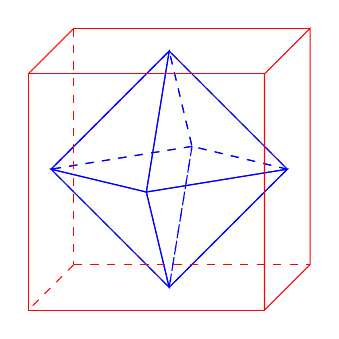
\begin{tikzpicture}[z = -5.5, scale = 1.5]
    \coordinate (O1) at (0, 0, -1);
    \coordinate (O2) at (-1, 0, 0);
    \coordinate (O3) at (0, 0, 1);
    \coordinate (O4) at (1, 0, 0);
    \coordinate (O5) at (0, 1, 0);
    \coordinate (O6) at (0, -1, 0);

    \draw [draw = blue, dashed] (O1) -- (O2) -- (O5) -- cycle;
    \draw [draw = blue, dashed] (O4) -- (O1) -- (O5) -- cycle;
    \draw [draw = blue, dashed] (O1) -- (O2) -- (O6) -- cycle;
    \draw [draw = blue, dashed] (O4) -- (O1) -- (O6) -- cycle;
    \draw [draw = blue] (O2) -- (O3) -- (O5) -- cycle;
    \draw [draw = blue] (O3) -- (O4) -- (O5) -- cycle;
    \draw [draw = blue] (O2) -- (O3) -- (O6) -- cycle;
    \draw [draw = blue] (O3) -- (O4) -- (O6) -- cycle;

    \coordinate (C1) at (-1, -1, -1);
    \coordinate (C2) at (-1, -1, 1);
    \coordinate (C3) at (-1, 1, 1);
    \coordinate (C4) at (-1, 1, -1);
    \coordinate (C5) at (1, -1, -1);
    \coordinate (C6) at (1, -1, 1);
    \coordinate (C7) at (1, 1, 1);
    \coordinate (C8) at (1, 1, -1);

    \draw [draw = red, dashed] (C1) -- (C2);
    \draw [draw = red] (C2) -- (C3);
    \draw [draw = red] (C3) -- (C4);
    \draw [draw = red, dashed] (C4) -- (C1);
    \draw [draw = red] (C5) -- (C6) -- (C7) -- (C8) -- cycle;
    \draw [draw = red, dashed] (C1) -- (C5);
    \draw [draw = red] (C2) -- (C6);
    \draw [draw = red] (C3) -- (C7);
    \draw [draw = red] (C4) -- (C8);
  \end{tikzpicture}
\end{center}

\subsection{Symmetries of the tetrahedron}
\subsubsection*{Rotations}
Let $1, 2, 3, 4$ be the vertices (in any order). $G^+$ is just the rotations. Let it act on the vertices. Then $\orb(1) = \{1, 2, 3, 4\}$ and $\stab(1) = \{$ rotations in the axis through 1 and the center of the opposite face $\} = \{e, \frac{2\pi}{3}, \frac{4\pi}{3}\}$

So $|G^+| = 4\cdot 3 = 12$ by the orbit-stabilizer theorem.

The action gives a group homomorphism $\varphi: G^+ \to S_4$. Clearly $\ker \varphi = \{e\}$. So $G^+ \leq S_4$ and $G^+$ has size 12. We ``guess'' it is $A_4$ (actually it \emph{must} be $A_4$ since that is the only subgroup of $S_4$ of order 12, but it's nice to see why that's the case).

If we rotate in an axis through 1, we get $(2\; 3\; 4), (2\; 4\; 3)$. Similarly, rotating through other axes through vertices gives all 3-cycles.

If we rotate through an axis that passes through two opposite edges, e.g.\ through 1-2 edge and 3-4 edge, then we have $(1\; 2)(3\; 4)$ and similarly we obtain all double transpositions. So $G^+ \cong A_4$. This shows that there is no \emph{rotation} that fixes two vertices and swaps the other two.

\subsubsection*{All symmetries}
Now consider the plane that goes through 1, 2 and the mid-point of 3 and 4. Reflection through this plane swaps 3 and 4, but doesn't change $1, 2$. So now $\stab(1) = \bra (2\; 3\; 4), (3, 4)\ket \cong D_6$ (alternatively, if we want to fix 1, we just move 2, 3, 4 around which is the symmetries of the triangular base)

So $|G| = 4\cdot 6 = 24$ and $G\cong S_4$ (which makes sense since we can move any of its vertices around in any way and still be a tetrahedron, so we have all permutations of vertices as the symmetry group)

\section{M\texorpdfstring{\"o}{o}bius group}
\subsection{M\texorpdfstring{\"o}{o}bius maps}
We want to study maps $f: \C \to \C$ in the form $f(z) = \frac{az + b}{cz + d}$ with $a, b, c, d\in \C$ and $ad - bc \not= 0$.

We impose $ad - bc\not= 0$ or else the map will be constant: for any $z, w\in \C$, $f(z) - f(w) = \frac{(az + b)(cw + d) - (aw + b)(cz + d)}{(cw + d)(cz + d)} = \frac{(ad - bc)(z - w)}{(cw + d)(cz + d)}$. If $ad - bc = 0$, then $f$ is constant and boring (more importantly, it will not be invertible).

If $c\not=0$, then $f(-\frac{d}{c})$ involves division by 0. So we add $\infty$ to $\C$ to form the extended complex plane (Riemann sphere) $\C\cup \{\infty\}= \C_\infty$ (cf.\ Vectors and Matrices). Then we define $f(-\frac{d}{c}) = \infty$. We call $\C_\infty$ a one-point compactification of $\C$ (because it adds one point to $\C$ to make it compact, cf.\ Metric and Topology).

\begin{defi}[M\"obius map]
  A \emph{M\"obius map} is a map from $\C_\infty \to \C_\infty$ of the form
  \[
    f(z) = \frac{az + b}{cz + d},
  \]
  where $a, b, c, d\in \C$ and $ad - bc\not= 0$, with $f(-\frac{d}{c}) = \infty$ and $f(\infty) = \frac{a}{c}$ when $c\not= 0$. (if $c = 0$, then $f(\infty)=\infty$)
\end{defi}

\begin{lemma}[M\"obius bijectivity]
  The M\"obius maps are bijections $\C_\infty \to \C_\infty$.
\end{lemma}

\begin{proof}
  The inverse of $f(z) = \frac{az + b}{cz+ d}$ is $g(z) = \frac{dz - b}{-cz + a}$, which we can check by composition both ways.
\end{proof}

\begin{prop}[M\"obius group]
  The M\"obius maps form a group $M$ under function composition. (The M\"obius group)
\end{prop}
\begin{proof}
  The group axioms are shown as follows:
  \begin{enumerate}[label=\arabic{*}.]
      \setcounter{enumi}{-1}
    \item If $f_1(z) = \frac{a_1z + b_1}{c_1z + d_1}$ and $f_2(z) = \frac{a_2z + b_2}{c_2 z + d_2}$, then $\displaystyle f_2\circ f_1 (z) = \frac{a_2\left(\frac{a_1z + b_1}{c_1z + d_1}\right) + b_2}{c_2\left(\frac{a_1z + b_1}{c_1z + d_1}\right) + d_2} = \frac{(a_1a_2 + b_2c_1)z + (a_2b_1 + b_2d_1)}{(c_2a_1 + d_2c_1)z + (c_2b_1 + d_1d_2)}$. Now we have to check that $ad - bc \not = 0$: we have $(a_1a_2 + b_2c_1)(c_2b_1 + d_1d_2) - (a_2b_1 + b_2d_1)(c_2a_1 + d_2c_1) = (a_1d_1 - b_1c_1)(a_2d_2 - b_2c_2)\not =0 $.

      (This works for $z\not= \infty, -\frac{d_1}{c_1}$. We have to manually check the special cases, which is simply yet more tedious algebra)
    \item The identity function is $1(z) = \frac{1z + 0}{0 + 1}$ which satisfies $ad - bc \not= 0$.
    \item We have shown above that $f^{-1}(z) = \frac{dz - b}{-cz + a}$ with $da - bc\not= 0$, which are also M\"obius maps
    \item Composition of functions is always associative
  \end{enumerate}
\end{proof}
$M$ is not abelian. e.g.\ $f_1(z) = 2z$ and $f_2(z) = z + 1$ are not commutative: $f_1\circ f_2(z) = 2z+2$ and $f_2\circ f_1(z) = 2z + 1$.

Note that the point at ``infinity'' is not special. $\infty$ is no different to any other point of the Riemann sphere. However, from the way we write down the M\"obius map, we have to check infinity specially. In this particular case, we can get quite far with conventions such as $\frac{1}{\infty} = 0$, $\frac{1}{0} = \infty$ and $\frac{a\cdot \infty}{c\cdot \infty} = \frac{a}{c}$.

Clearly $\frac{az + b}{cz + d} = \frac{\lambda az + \lambda b}{\lambda cz + \lambda d}$ for any $\lambda \not= 0$. So we do not have a unique representation of a map in terms of $a, b, c, d$. But $a, b, c, d$ does uniquely determine a M\"obius map.

\begin{prop}[$\GL_2(\C)$ to M\"obius group homomorphism]
  The map $\theta: \GL_2(\C)\to M$ sending $
  \displaystyle \begin{pmatrix}
    a & b\\
    c & d
  \end{pmatrix} \mapsto \frac{az + b}{cz + d}$ is a surjective group homomorphism.
\end{prop}

\begin{proof}
  Firstly, since the determinant $ad - bc$ of any matrix in $\GL_2(\C)$ is non-zero, it does map to a M\"obius map. This also shows that $\theta$ is surjective.

  We have previously calculated that
  \[
    \theta(A_2)\circ \theta(A_1) = \frac{(a_1a_2 + b_2c_1)z + (a_2b_1 + b_2d_1)}{(c_2a_1 + d_2c_1)z + (c_2b_1 + d_1d_2)} = \theta(A_2A_1)
  \]
  So it is a homomorphism.
\end{proof}

The kernel of $\theta$ is
\[
  \ker(\theta) = \left\{A\in \GL_2(\C): (\forall z)\,z = \frac{az + b}{cz + d}\right\}
\]
We can try different values of $z$: $z = \infty \Rightarrow c = 0$; $z = 0 \Rightarrow b = 0$; $z = 1\Rightarrow d = a$. So
\[
  \ker\theta = Z = \{\lambda I: \lambda \in \C, \lambda\not= 0\},
\]
where $I$ is the identity matrix and $Z$ is the centre of $\GL_2(\C)$.

By the isomorphism theorem, we have
\[
  M \cong \GL_2(\C)/Z
\]

\begin{defi}[Projective general linear group $\mathrm{PGL}_2(\C)$]
  (Non-examinable) The projective general linear group is
  \[
    \mathrm{PGL}_2(\C) = \GL_2(\C)/Z.
  \]
\end{defi}
Since $f_A = f_B$ iff $B = \lambda A$ for some $\lambda\not= 0$ (where $A, B$ are the corresponding matrices of the maps), if we restrict $\theta$ to $\SL_2(\C)$, we have $\left.\theta\right|_{\SL_2(\C)}: \SL_2(\C)\to M$ is also surjective. The kernel is now just $\{\pm I\}$. So
\[
  M \cong \SL_2(\C)/\{\pm I\} = \mathrm{PSL_2}(\C)
\]
Clearly $\mathrm{PSL}_2(\C)\cong \mathrm{PGL}_2(\C)$ since both are isomorphic to the M\"obius group.

\begin{prop}[M\"obius map generators]
  Every M\"obius map is a composite of maps of the following form:
  \begin{enumerate}
    \item Dilation/rotation: $f(z) = az$, $a\not= 0$
    \item Translation: $f(z) = z + b$
    \item Inversion: $f(z) = \frac{1}{z}$
  \end{enumerate}
\end{prop}
\begin{proof}
  Let $\frac{az + b}{cz + d}\in M$.

  If $c = 0$, i.e.\ $g(\infty) = \infty$, then $g(z) = \frac{a}{d}z + \frac{b}{d}$, i.e.
  \[
    z\mapsto \frac{a}{d} z\mapsto \frac{a}{d}z + \frac{b}{d}.
  \]
  If $c\not= 0$, let $g(\infty)=z_0$, Let $h(z) = \frac{1}{z - z_0}$. Then $hg(\infty) = \infty$ is of the above form. We have $h^{-1}(w) = \frac{1}{w} + z_0$being of type (iii) followed by (ii). So $g = h^{-1} (hg)$ is a composition of maps of the three forms listed above.

  Alternatively, with sufficient magic, we have
  \[
    z\mapsto z + \frac{d}{c} \mapsto \frac{1}{z + \frac{d}{c}} \mapsto -\frac{ad + bc}{c^2(z + \frac{d}{c})}\mapsto \frac{a}{c} -\frac{ad + bc}{c^2(z + \frac{d}{c})} = \frac{az + b}{cz + d}.\qedhere
  \]
\end{proof}
Note that the non-calculation method above can be transformed into another (different) composition with the same end result. So the way we compose a M\"obius map from the ``elementary'' maps are not unique.

\subsection{Fixed points of M\texorpdfstring{\"o}{o}bius maps}
\begin{defi}[Fixed point]
  A \emph{fixed point} of $f$ is a $z$ such that $f(z) = z$.
\end{defi}

We know that any M\"obius map with $c = 0$ fixes $\infty$. We also know that $z\to z + b$ for any $b\not= 0$ fixes $\infty$ only, where as $z\mapsto az$ for $a\not= 0, 1$ fixes $0$ and $\infty$. It turns out that you cannot have more than two fixed points, unless you are the identity.

\begin{prop}[Three fixed points rigidity]
  Any M\"obius map with at least 3 fixed points must be the identity.
\end{prop}

\begin{proof}
  Consider $f(z) = \frac{az + b}{cz + d}$. This has fixed points at those $z$ which satisfy $\frac{az + b}{cz + d} = z \Leftrightarrow cz^2 + (d - a)z - b = 0$. A quadratic has at most two roots, unless $c = b = 0$ and $d = a$, in which the equation just says $0 = 0$.

  However, if $c = b= 0$ and $d = a$, then $f$ is just the identity.
\end{proof}

\begin{prop}[M\"obius map normal form]
  Any M\"obius map is conjugate to $f(z) = \nu z$ for some $\nu\not= 0$ or to $f(z) = z + 1$.
\end{prop}

\begin{proof}
  We have the surjective group homomorphism $\theta: \GL_2(\C) \to M$. The conjugacy classes of $\GL_2(\C)$ are of types
  \begin{align*}
    \begin{pmatrix}
      \lambda & 0\\
      0 & \mu
    \end{pmatrix} &\mapsto g(z) = \frac{\lambda z + 0}{0z + \mu} = \frac{\lambda}{\mu}z\\
    \begin{pmatrix}
      \lambda & 0\\
      0 & \lambda
    \end{pmatrix} &\mapsto g(z) = \frac{\lambda z + 0}{0z + \lambda} = 1 z\\
    \begin{pmatrix}
      \lambda & 1\\
      0 & \lambda
    \end{pmatrix} &\mapsto g(z) = \frac{\lambda z + 1}{\lambda} = z + \frac{1}{\lambda}
  \end{align*}
  But the last one is not in the form $z + 1$. We know that the last $g(z)$ can also be represented by $
  \begin{pmatrix}
    1 & \frac{1}{\lambda}\\
    0 & 1
  \end{pmatrix}$, which is conjugate to $
  \begin{pmatrix}
    1 & 1\\
    0 & 1
  \end{pmatrix}$ (since that's its Jordan-normal form). So $z + \frac{1}{\lambda}$ is also conjugate to $z + 1$.
\end{proof}

Now we see easily that (for $\nu \not= 0, 1$), $\nu z$ has $0$ and $\infty$ as fixed points, $z + 1$ only has $\infty$. Does this transfer to their conjugates?

\begin{prop}[M\"obius map fixed point count]
  Every non-identity has exactly 1 or 2 fixed points.
\end{prop}

\begin{proof}
  Given $f\in M$ and $f\not= \mathrm{id}$. So $\exists h\in M$ such that $hfh^{-1}(z) = \nu{z}$. Now $f(w) = w \Leftrightarrow hf(w) = h(w) \Leftrightarrow hfh^{-1}(h(w)) = h(w)$. So $h(w)$ is a fixed point of $hfh^{-1}$. Since $h$ is a bijection, $f$ and $hfh^{-1}$ have the same number of fixed points.

  So $f$ has exactly $2$ fixed points if $f$ is conjugate to $\nu z$, and exactly 1 fixed point if $f$ is conjugate to $z + 1$.
\end{proof}
Intuitively, we can show that conjugation preserves fixed points because if we conjugate by $h$, we first move the Riemann sphere around by $h$, apply $f$ (that fixes the fixed points) then restore the Riemann sphere to its original orientation. So we have simply moved the fixed point around by $h$.

\subsection{Permutation properties of M\texorpdfstring{\"o}{o}bius maps}
We have seen that the M\"obius map with three fixed points is the identity. As a corollary, we obtain the following.

\begin{prop}[Three-point determination]
  Given $f, g\in M$. If $\exists z_1, z_2, z_3\in \C_{\infty}$ such that $f(z_i) = g(z_i)$, then $f = g$. i.e.\ every M\"obius map is uniquely determined by three points.
\end{prop}

\begin{proof}
  As M\"obius maps are invertible, write $f(z_i) = g(z_i)$ as $g^{-1}f(z_i) = z_i$. So $g^{-1}f$ has three fixed points. So $g^{-1}f$ must be the identity. So $f = g$.
\end{proof}

\begin{defi}[Three-transitive action]
  An action of $G$ on $X$ is called \emph{three-transitive} if the induced action on $\{(x_1, x_2, x_3)\in X^3: x_i\text{ pairwise disjoint}\}$, given by $g(x_1, x_2, x_3) = (g(x_1), g(x_2), g(x_3))$, is transitive.

  This means that for any two triples $x_1, x_2, x_3$ and $y_1, y_2, y_3$ of distinct elements of $X$, there exists $g\in G$ such that $g(x_i) = y_i$.

  If this $g$ is always unique, then the action is called \emph{sharply three transitive}
\end{defi}
This is a really weird definition. The reason we raise it here is that the M\"obius map satisfies this property.

\begin{prop}[Sharp three-transitivity of $M$]
  The M\"obius group $M$ acts sharply three-transitively on $\C_\infty$.
\end{prop}

\begin{proof}
  We want to show that we can send any three points to any other three points. However, it is easier to show that we can send any three points to $0, 1, \infty$.

  Suppose we want to send $z_1\to \infty, z_2\mapsto 0, z_3 \mapsto 1$. Then the following works:
  \[
    f(z) = \frac{(z - z_2)(z_3 - z_1)}{(z - z_1)(z_3 - z_2)}
  \]
  If any term $z_i$ is $\infty$, we simply remove the terms with $z_i$, e.g.\ if $z_1 = \infty$, we have $f(z) = \frac{z - z_2}{z_3 - z_2}$.

  So given also $w_1, w_2, w_3$ distinct in $\C_\infty$ and $g\in M$ sending $w_1\mapsto \infty, w_2\mapsto 0, w_3\mapsto 1$, then we have $g^{-1}f(z_i) = w_i$.

  The uniqueness of the map follows from the fact that a M\"obius map is uniquely determined by 3 points.
\end{proof}

3 points not only define a M\"obius map uniquely. They also uniquely define a line or circle. Note that on the Riemann sphere, we can think of a line as a circle through infinity, and it would be technically correct to refer to both of them as ``circles''. However, we would rather be clearer and say ``line/circle''.

We will see how M\"obius maps relate to lines and circles. We will first recap some knowledge about lines and circles in the complex plane.

\begin{lemma}[Circle and line equation in $\C$]
  The general equation of a circle or straight line in $\C$ is
  \[
    Az\bar z + \bar Bz + B\bar z + C = 0,
  \]
  where $A, C\in \R$ and $|B|^2 > AC$.
\end{lemma}
$A = 0$ gives a straight line. If $A \not= 0, B = 0$, we have a circle centered at the origin. If $C = 0$, the circle passes through 0.

\begin{proof}
  This comes from noting that $|z - B| = r$ for $r \in \R> 0$ is a circle; $|z - a| = |z - b|$ with $a\not= b $ is a line. The detailed proof can be found in Vectors and Matrices.
\end{proof}

\begin{prop}[Circle preservation]
  M\"obius maps send circles/straight lines to circles/straight lines. Note that it can send circles to straight lines and vice versa.

  Alternatively, M\"obius maps send circles on the Riemann sphere to circles on the Riemann sphere.
\end{prop}

\begin{proof}
  We can either calculate it directly using $w = \frac{az + b}{cz + d}\Leftrightarrow z = \frac{dw - b}{-cw + a}$ and substituting $z$ into the circle equation, which gives $A' w\bar w + \bar B' w + B'\bar w + C' = 0$ with $A', C'\in \R$.

  Alternatively, we know that each M\"obius map is a composition of translation, dilation/rotation and inversion. We can check for each of the three types. Clearly dilation/rotation and translation maps a circle/line to a circle/line. So we simply do inversion: if $w = z^{-1}$
  \begin{align*}
    &\; Az\bar z + \bar Bz + B\bar z + C = 0\\
    \Leftrightarrow &\; Cw\bar w + Bw + \bar B\bar w + A = 0\qedhere
  \end{align*}
\end{proof}

\begin{eg}
  Consider $f(z) = \frac{z - i}{z + i}$. Where does the real line go? The real line is simply a circle through $0, 1, \infty$. $f$ maps this circle to the circle containing $f(\infty) = 1$, $f(0) = -1$ and $f(1) = -i$, which is the unit circle.

  Where does the upper half plane go? We know that the M\"obius map is smooth. So the upper-half plane either maps to the inside of the circle or the outside of the circle. We try the point $i$, which maps to $0$. So the upper half plane is mapped to the inside of the circle.
\end{eg}
\subsection{Cross-ratios}
  Finally, we'll look at an important concept known as \emph{cross-ratios}. Roughly speaking, this is a quantity that is preserved by M\"obius transforms.

\begin{defi}[Cross-ratios]
  Given four distinct points $z_1, z_2, z_3, z_4\in \C_\infty,$ their \emph{cross-ratio} is $[z_1, z_2, z_3, z_4] = g(z_4)$, with $g$ being the unique M\"obius map that maps $z_1\mapsto \infty, z_2\mapsto 0, z_3\mapsto 1$. So $[\infty, 0, 1, \lambda] = \lambda$ for any $\lambda\not= \infty, 0, 1$. We have
  \[
    [z_1, z_2, z_3, z_4] = \frac{z_4 - z_2}{z_4 - z_1} \cdot \frac{z_3 - z_1}{z_3 - z_2}
  \]
  (with special cases as above).
\end{defi}
We know that this exists and is uniquely defined because $M$ acts sharply three-transitively on $\C_\infty$.

Note that different authors use different permutations of $1, 2, 3, 4$, but they all lead to the same result as long as you are consistent.

\begin{lemma}[Cross-ratio double transposition symmetry]
  For $z_1, z_2, z_3, z_4\in \C_\infty$ all distinct, then
  \[
    [z_1, z_2, z_3, z_4] = [z_2, z_1, z_4, z_3] = [z_3, z_4, z_1, z_2] = [z_4, z_3, z_2, z_1]
  \]
  i.e.\ if we perform a double transposition on the entries, the cross-ratio is retained.
\end{lemma}

\begin{proof}
  By inspection of the formula.
\end{proof}

\begin{prop}[Cross-ratio invariance]
  If $f\in M$, then $[z_1, z_2, z_3, z_4] = [f(z_1), f(z_2), f(z_3), f(z_4)]$.
\end{prop}

\begin{proof}
  Use our original definition of the cross ratio (instead of the formula). Let $g$ be the unique M\"obius map such that $[z_1, z_2, z_3, z_4] = g(z_4) = \lambda$, i.e.
  \begin{align*}
    z_1 &\xmapsto{g} \infty\\
    z_2 &\mapsto 0\\
    z_3 &\mapsto 1\\
    z_4 &\mapsto \lambda
  \end{align*}
  We know that $gf^{-1}$ sends
  \begin{align*}
    f(z_1)\xmapsto{f^{-1}} z_1 &\xmapsto{g} \infty\\
    f(z_2)\xmapsto{f^{-1}} z_2 &\xmapsto{g} 0\\
    f(z_3)\xmapsto{f^{-1}} z_3 &\xmapsto{g} 1\\
    f(z_4)\xmapsto{f^{-1}} z_4 &\xmapsto{g} \lambda
  \end{align*}
  So $[f(z_1), f(z_2), f(z_3), f(z_4)] = gf^{-1}f(z_4) = g(z_4) = \lambda$.
\end{proof}

In fact, we can see from this proof that: given $z_1, z_2, z_3, z_4$ all distinct and $w_1, w_2, w_3, w_4$ distinct in $\C_\infty$, then $\exists f\in M$ with $f(z_i) = w_i$ iff $[z_1, z_2, z_3, z_4] = [w_1, w_2, w_3, w_4]$.

\begin{cor}[Concyclic criterion]
  $z_1, z_2, z_3, z_4$ lie on some circle/straight line iff $[z_1, z_2, z_3, z_4]\in \R$.
\end{cor}

\begin{proof}
  Let $C$ be the circle/line through $z_1, z_2, z_3$. Let $g$ be the unique M\"obius map with $g(z_1) = \infty$, $g(z_2) = 0$, $g(z_3) = 1$. Then $g(z_4) = [z_1, z_2, z_3, z_4]$ by definition.

  Since we know that M\"obius maps preserve circle/lines, $z_4\in C \Leftrightarrow g(z_4)$ is on the line through $\infty, 0, 1$, i.e.\ $g(z_4) \in \R$.
\end{proof}

\section{Projective line (non-examinable)}
We have seen in matrix groups that $\GL_2(\C)$ acts on $\C^2$, the column vectors. Instead, we can also have $\GL_2(\C)$ acting on the set of 1-dimensional subspaces (i.e.\ lines) of $\C^2$.

For any $\mathbf{v}\in \C^2$, write the line generated by $\mathbf{v}$ as $\bra \mathbf{v}\ket$. Then clearly $\bra \mathbf{v} \ket = \{\lambda \mathbf{v}: \lambda\in \C\}$. Now for any $A\in \GL_2(\C)$, define the action as $A\bra \mathbf{v}\ket = \bra A\mathbf{v}\ket$. Check that this is well-defined: for any $\bra \mathbf{v} \ket = \bra \mathbf{w}\ket$, we want to show that $\bra A\mathbf{v}\ket = \bra A\mathbf{w}\ket$. This is true because $\bra \mathbf{v} \ket = \bra \mathbf{w}\ket$ if and only if $\mathbf{w} = \lambda \mathbf{v}$ for some $\lambda\in \C\setminus\{0\}$, and then $\bra A\mathbf{w}\ket = \bra A\lambda\mathbf{v}\ket = \bra \lambda (A\mathbf{v})\ket = \bra A\mathbf{v}\ket$.

What is the kernel of this action? By definition the kernel has to fix all lines. In particular, it has to fix our magic lines generated by $\binom{1}{0}, \binom{0}{1}$ and $\binom{1}{1}$. Since we want $A\bra \binom{1}{0}\ket = \bra \binom{1}{0}\ket$, so we must have $A\binom{1}{0} = \binom{\lambda}{0}$ for some $\lambda$. Similarly, $A\binom{0}{1} = \binom{0}{\mu}$. So we can write $A =
\begin{pmatrix}
  \lambda & 0\\
  0 & \mu
\end{pmatrix}$. However, also need $A\bra \binom{1}{1}\ket = \bra\binom{1}{1}\ket$. Since $A$ is a linear function, we know that $A \binom{1}{1} = A \binom{1}{0} + A \binom{0}{1} = \binom{\lambda }{\mu}$. For the final vector to be parallel to $\binom{1}{1}$, we must have $\lambda = \mu$. So $A = \lambda I$ for some $I$. Clearly any matrix of this form fixes any line. So the kernel $Z = \{\lambda I: \lambda\in \C\setminus\{0\}\}$.

Note that every line is uniquely determined by its slope. For any $\mathbf{v} = (v_1, v_2), \mathbf{w} = (w_1, w_2)$, we have $\bra \mathbf{v}\ket = \bra \mathbf{w}\ket$ iff $z_1/z_2 = w_1/w_2$. So we have a one-to-one correspondence from our lines to $\C_\infty$, that maps $\bra \binom{z_1}{z_2}\ket\leftrightarrow z_1/z_2$.

Finally, for each $A\in \GL_2(\C)$, given any line $\bra \binom{z}{1}\ket$, we have
\[
  \begin{pmatrix}
    a & b\\
    c & d
  \end{pmatrix}
  \left\bra
  \begin{pmatrix}
    z\\1
  \end{pmatrix}\right\ket = \left\bra
  \begin{pmatrix}
    az + b\\
    cz + d
  \end{pmatrix}
  \right\ket \leftrightarrow \frac{az + b}{cz + d}
\]
So $\GL_2(\C)$ acting on the lines is just ``the same'' as the M\"obius groups acting on points.
\end{document}
